% ============================================================================
% LeakLens -- OSINT Intelligence Platform for Leaked Data Research
% PFA Report -- iTeam University 2025/2026
% ============================================================================
\documentclass[12pt,a4paper,oneside]{report}

% ---- Encoding & language ---------------------------------------------------
\usepackage[utf8]{inputenc}
\usepackage[T1]{fontenc}
\usepackage[english]{babel}

% ---- Page geometry ---------------------------------------------------------
\usepackage[
  top=2.5cm, bottom=2.5cm,
  left=2.5cm, right=2.5cm,
  headheight=15pt
]{geometry}

% ---- Fonts -----------------------------------------------------------------
\usepackage{lmodern}
\usepackage{microtype}

% ---- Graphics & colors -----------------------------------------------------
\usepackage{graphicx}
\graphicspath{{figures/}{./figures/}}
\DeclareGraphicsExtensions{.png,.pdf,.jpg,.jpeg}
\usepackage{grffile}
\usepackage{adjustbox}
\usepackage[dvipsnames,svgnames,table]{xcolor}
\usepackage{tikz}
\usetikzlibrary{shapes,arrows.meta,positioning,calc,fit,backgrounds}

% Brand colours (cyber theme)
\definecolor{CyberNavy}{HTML}{0B1F3A}
\definecolor{CyberTeal}{HTML}{00B4D8}
\definecolor{CyberAccent}{HTML}{0077B6}
\definecolor{CoverRed}{HTML}{C0392B}

% ---- Tables ----------------------------------------------------------------
\usepackage{booktabs}
\usepackage{tabularx}
\usepackage{multirow}
\usepackage{array}
\newcolumntype{L}[1]{>{\raggedright\arraybackslash}p{#1}}
\newcolumntype{C}[1]{>{\centering\arraybackslash}p{#1}}

% ---- Code listings ---------------------------------------------------------
\usepackage{listings}
\definecolor{codebg}{HTML}{F5F5F5}
\definecolor{codeframe}{HTML}{CCCCCC}
\definecolor{keyword}{HTML}{0000FF}
\definecolor{comment}{HTML}{6A9955}
\definecolor{string}{HTML}{A31515}

\lstset{
  backgroundcolor=\color{codebg},
  frame=single,
  rulecolor=\color{codeframe},
  basicstyle=\small\ttfamily,
  keywordstyle=\color{keyword}\bfseries,
  commentstyle=\color{comment}\itshape,
  stringstyle=\color{string},
  breaklines=true,
  breakatwhitespace=true,
  numbers=left,
  numberstyle=\tiny\color{gray},
  numbersep=8pt,
  tabsize=2,
  showstringspaces=false,
  captionpos=b,
  aboveskip=10pt,
  belowskip=10pt,
}

\lstdefinelanguage{yaml}{
  keywords={true,false,null},
  sensitive=false,
  comment=[l]{\#},
  morestring=[b]',
  morestring=[b]",
}

% ---- Headers & footers -----------------------------------------------------
\usepackage{fancyhdr}
\pagestyle{fancy}
\fancyhf{}
\fancyhead[L]{\small\leftmark}
\fancyhead[R]{\small LeakLens --- PFA 2025--2026}
\fancyfoot[C]{\thepage}
\renewcommand{\headrulewidth}{0.4pt}
\renewcommand{\footrulewidth}{0pt}

\fancypagestyle{plain}{
  \fancyhf{}
  \fancyfoot[C]{\thepage}
  \renewcommand{\headrulewidth}{0pt}
}

% ---- Hyperlinks ------------------------------------------------------------
\usepackage[
  colorlinks=true,
  linkcolor=NavyBlue,
  citecolor=ForestGreen,
  urlcolor=RoyalBlue,
  bookmarks=true,
  pdfauthor={Motez Machghoul},
  pdftitle={LeakLens -- OSINT Intelligence Platform},
  pdfsubject={PFA Report -- iTeam University 2025/2026},
]{hyperref}

% ---- Captions --------------------------------------------------------------
\usepackage[font=small,labelfont=bf]{caption}

% ---- Bibliography ----------------------------------------------------------
\usepackage[numbers,sort&compress]{natbib}

% ---- Misc ------------------------------------------------------------------
\usepackage{float}
\usepackage{placeins}
\usepackage{enumitem}
\usepackage{parskip}
\usepackage{longtable}
\usepackage{setspace}
\onehalfspacing

% ---- Custom commands -------------------------------------------------------
\newcommand{\leaklens}{\textsc{LeakLens}}
\newcommand{\theplatform}{the platform}
\newcommand{\tikzfig}[1]{\begin{center}\adjustbox{width=0.92\linewidth,center}{#1}\end{center}}
\newcommand{\logobox}[2]{\raisebox{-0.4\height}{\includegraphics[height=#1]{#2}}}
\newcommand{\iteamlogo}{%
  \IfFileExists{figures/iteam-logo.png}{%
    
\includegraphics[height=2.4cm]{iteam-logo.png}%
  }{%
    
\begin{tikzpicture}
      \node[draw=CyberTeal,rounded corners=4pt,minimum width=4.2cm,
        minimum height=2.2cm,font=\bfseries\large,text=CyberNavy]
        {iTeam University};
    \end{tikzpicture}%
  }%
}
\newcommand{\figref}[1]{Figure~\ref{#1}}
\newcommand{\tabref}[1]{Table~\ref{#1}}
\newcommand{\chapref}[1]{Chapter~\ref{#1}}
\newcommand{\secref}[1]{Section~\ref{#1}}
\newcommand{\chmark}{\ding{51}}
\newcommand{\xmark}{\ding{55}}
\usepackage{pifont}
\newcommand{\cmark}{\ding{51}}

% ============================================================================
\begin{document}

% ---- Front matter ----------------------------------------------------------
\pagenumbering{roman}
% ============================================================================
% Front matter
% ============================================================================

% ----------------------------------------------------------------------------
% Cover page
% ----------------------------------------------------------------------------
\begin{titlepage}
\thispagestyle{empty}
\pagecolor{white}

\begin{tikzpicture}[remember picture,overlay]
  % Thin red vertical accent (left margin)
  \draw[CoverRed,line width=1.2pt]
    ([xshift=1.6cm]current page.north west) --
    ([xshift=1.6cm]current page.south west);
\end{tikzpicture}

% ---- Header ----------------------------------------------------------------
\noindent
\begin{minipage}[t]{0.42\textwidth}
  \vspace{0pt}
  \iteamlogo
\end{minipage}%
\hfill
\begin{minipage}[t]{0.52\textwidth}
  \vspace{0pt}
  \raggedleft
  \setlength{\fboxsep}{6pt}
  \fbox{%
    \parbox[c][1.1cm][c]{0.94\linewidth}{%
      \centering\small\bfseries
      RAPPORT DE PROJET DE FIN D'ANN\'EES%
    }%
  }\\[6pt]
  {\scriptsize Département Génie Informatique --- Cybersecurity}
\end{minipage}

\vspace{0.55cm}
\noindent{\color{CoverRed}\rule{\textwidth}{0.8pt}}

\vspace{1.4cm}

% ---- Main title block ------------------------------------------------------
\noindent\hspace{1.15cm}%
\begin{minipage}[t]{0.88\textwidth}
  {\fontsize{46}{50}\selectfont\bfseries\rmfamily \leaklens{}}\\[0.55cm]
  {\Large\color{CoverRed}\bfseries
    OSINT Intelligence Platform\\[0.12cm]
    for Leaked Data Research}\\[0.45cm]
  {\normalsize
    Full-stack breach search deployed on Vercel and VPS
    (FastAPI, Next.js, PostgreSQL, Snusbase)}\\[1.4cm]
  \setlength{\fboxsep}{8pt}
  \fbox{%
    \parbox{0.72\textwidth}{%
      \centering
      Spécialité~: \textbf{Cybersecurity}%
    }%
  }
\end{minipage}

\vfill

% ---- Academic year (left) + author block (right) -----------------------------
\noindent
\begin{minipage}[b]{0.28\textwidth}
  \hspace{1.15cm}
  {\scriptsize Année Universitaire}\\[2pt]
  {\Large\bfseries 2025 / 2026}
\end{minipage}%
\hfill
\begin{minipage}[b]{0.68\textwidth}
  \raggedleft
  \renewcommand{\arraystretch}{1.35}
  \begin{tabular}{@{} >{\raggedright\arraybackslash}p{0.31\linewidth}
                     >{\raggedright\arraybackslash}p{0.34\linewidth}
                     >{\raggedright\arraybackslash}p{0.28\linewidth} @{}}
    \textbf{Réalisé par~:} &
    \textbf{Encadré par~:} &
    \textbf{Soutenu en~:} \\[2pt]
    Motez Machghoul &
    Mr Raihane Modhaffer &
    Juin 2026 \\
  \end{tabular}
\end{minipage}

\vspace*{1.6cm}
\end{titlepage}
\nopagecolor

% ----------------------------------------------------------------------------
% Dedication
% ----------------------------------------------------------------------------
\clearpage
\thispagestyle{empty}
\vspace*{2.5cm}
\begin{center}
  {\LARGE\bfseries Dedication}
\end{center}
\vspace{1.5cm}
\begin{flushright}
\begin{minipage}{0.58\textwidth}
\large\itshape

To my parents,\\
for their unconditional love and support\\
that made this journey possible.\\[14pt]

To my friends and colleagues,\\
who shared the challenges and rewards\\
of this academic adventure.\\[14pt]

To everyone working to make the digital world safer.\\[20pt]

\normalfont\normalsize
\textit{Motez Machghoul}
\end{minipage}
\end{flushright}
\clearpage

% ----------------------------------------------------------------------------
% Acknowledgments
% ----------------------------------------------------------------------------
\chapter*{Acknowledgments}
\addcontentsline{toc}{chapter}{Acknowledgments}

At the conclusion of this end-of-year project, I wish to express my sincere
gratitude to everyone who contributed to the realization of this work.

I would first like to thank \textbf{Mr~Raihane Modhaffer}, my academic
supervisor, whose guidance, availability, and rigorous follow-up throughout
the project were decisive. His vision of modern cybersecurity challenges
shaped the technical direction of this report.

I warmly thank \textbf{iTeam University} and the teaching staff for the
quality of education provided---courses in software engineering, network
security, and information systems formed the foundation of this work.

My gratitude also goes to the open-source communities behind
\textbf{FastAPI}, \textbf{Next.js}, \textbf{Docker}, and \textbf{PostgreSQL},
whose documentation and tools made this project possible.

Finally, I thank my family for their patience and encouragement.

\vspace{1cm}
\noindent\textit{Motez Machghoul}\\
iTeam University, 2025--2026

\clearpage

% ----------------------------------------------------------------------------
% Summary (English)
% ----------------------------------------------------------------------------
\chapter*{Summary}
\addcontentsline{toc}{chapter}{Summary}

This report presents \leaklens{}, an Open-Source Intelligence (OSINT)
platform for breach-data research, developed as an End-of-Year Project at
iTeam University. The system allows authorized analysts to query compromised
records by email, username, IP address, password, name, hash, or domain, and
returns credential exposure details enriched with supplementary context from
public APIs.

The solution combines \textbf{Next.js~15} on Vercel for the web interface,
\textbf{FastAPI} and \textbf{PostgreSQL~16} on a VPS for the API layer, and
\textbf{Snusbase} as the primary breach-data provider. Access control relies
on JWT authentication, role-based permissions, invite-only registration, and
rate limiting. HTTP hardening includes CSP, HSTS, and strict CORS policies.

The main contribution is twofold: a practical OSINT search tool for exposure
assessment, and a working example of secure full-stack engineering applied
to a sensitive use case.

\textbf{Keywords:} OSINT, breach data, credential exposure, JWT, RBAC,
FastAPI, Next.js, Docker, Snusbase, PostgreSQL.

\clearpage

% ----------------------------------------------------------------------------
% List of abbreviations (project-relevant only)
% ----------------------------------------------------------------------------
\chapter*{List of Abbreviations}
\addcontentsline{toc}{chapter}{List of Abbreviations}

\noindent
Abbreviations used in this report.

\vspace{0.5cm}
\renewcommand{\arraystretch}{1.35}
\begin{longtable}{@{} l L{10.5cm} @{}}
\toprule
\textbf{Abbreviation} & \textbf{Definition} \\
\midrule
\endhead
API   & Application Programming Interface \\
CORS  & Cross-Origin Resource Sharing \\
CSP   & Content Security Policy \\
FK    & Foreign Key (database reference) \\
HSTS  & HTTP Strict Transport Security \\
HTTPS & HyperText Transfer Protocol Secure \\
JWT   & JSON Web Token \\
ORM   & Object-Relational Mapping \\
OSINT & Open-Source Intelligence \\
PII   & Personally Identifiable Information \\
PFA   & Projet de Fin d'Ann\'ees (End-of-Year Project) \\
RBAC  & Role-Based Access Control \\
REST  & REpresentational State Transfer \\
SQL   & Structured Query Language \\
SSR   & Server-Side Rendering \\
TLS   & Transport Layer Security \\
UUID  & Universally Unique Identifier \\
VPS   & Virtual Private Server \\
WHOIS & Protocol for querying domain and IP registration records \\
XSS   & Cross-Site Scripting \\
\bottomrule
\end{longtable}

\clearpage


\tableofcontents
\listoffigures
\listoftables
\clearpage

% ---- Main body -------------------------------------------------------------
\pagenumbering{arabic}
% ============================================================================
% Chapter I -- Preliminary Study
% ============================================================================

% ----------------------------------------------------------------------------
% Introduction G\'en\'erale (unnumbered, before Chapter I)
% ----------------------------------------------------------------------------
\chapter*{General Introduction}
\addcontentsline{toc}{chapter}{General Introduction}
\markboth{General Introduction}{}

The digital era has brought unprecedented connectivity---and with it, an
equally unprecedented exposure of sensitive data. According to industry
estimates, over 26~billion records were exposed in data breaches during 2023
alone, and the trend has only accelerated since~\cite{ibm-breach-report}. Every
month, new breach compilations, stealer logs, and combolists surface on
darknet forums, paste sites, and Telegram channels, making personally
identifiable information (PII) and credentials available to threat actors at
an industrial scale.

In response, a discipline known as \textbf{Open-Source Intelligence (OSINT)}
has emerged as a critical capability for cybersecurity defenders. OSINT
platforms allow analysts to search leaked data proactively---not to exploit it,
but to assess exposure, notify affected parties, and harden defenses before
attackers strike. Commercial platforms such as IntelligenceX, DeHashed, and
Snusbase provide this capability, but they are often expensive, opaque in
their architecture, and inaccessible to students and small security teams.

It is in this context that \leaklens{} was conceived: an OSINT intelligence
platform that enables authorized security researchers to search breached
databases by email, username, IP address, password, name, hash, or domain.
Results include credential exposure records enriched with supplementary
intelligence from public APIs. The project also demonstrates defensive
software engineering---hardening the application itself against common web
attacks.

This report documents the full engineering cycle, with emphasis on:

\begin{itemize}[nosep]
  \item The cybersecurity context and need for accessible OSINT tooling;
  \item Functional and non-functional requirements;
  \item Security-oriented architecture (JWT, RBAC, rate limiting, CSP);
  \item Production realization on Vercel and a VPS.
\end{itemize}

The report is organized in four chapters. \chapref{chap:preliminary} presents
the preliminary study, analyzes existing solutions, and justifies the choices
made. \chapref{chap:requirements} details the functional requirements and
technology stack. \chapref{chap:architecture}, the core of this report,
describes the security-oriented architecture design.
Finally, \chapref{chap:implementation} demonstrates the concrete realization
through screenshots and production metrics.

\clearpage

% ============================================================================
\chapter{Preliminary Study}
\label{chap:preliminary}
% ============================================================================

\section*{Introduction}

Before designing any technical solution, it is essential to understand the
context in which it operates, to analyze the tools already available on the
market, and to identify the gaps that the project aims to fill. This first
chapter establishes the foundations of the project: its context, problem
statement, and value for cybersecurity research.

% ----------------------------------------------------------------------------
\section{General Context}
\label{sec:context}
% ----------------------------------------------------------------------------

\subsection{The Cybersecurity Landscape (2024--2026)}

Between 2024 and 2026, the volume and \emph{reuse} of leaked breach data
became a defining feature of the threat landscape. Incidents no longer end
when a company publishes a breach notification---the stolen records live on
independently, copied into combolists, stealer-log archives, and searchable
databases traded on criminal forums, Telegram channels, and paste sites.

Several trends illustrate the scale of the problem:

\begin{itemize}[nosep]
  \item \textbf{2024 --- aggregation at industrial scale:} The ``Mother of All
        Breaches'' (MOAB) consolidated an estimated 26~billion records from
        dozens of prior incidents into a single searchable corpus, proving
        that breach data is permanently recycled rather than
        contained~\cite{moab}.
  \item \textbf{2025 --- stealer logs as a primary source:} Infostealer
        malware families (RedLine, Raccoon, Vidar, Lumma) harvest
        browser-saved credentials, session cookies, and autofill data from
        infected machines. These \emph{stealer logs} are sold in bulk and
        often contain live session tokens, making them more dangerous than
        static password dumps from older database breaches.
  \item \textbf{2026 --- sustained corporate and public-sector impact:}
        Healthcare providers, financial institutions, and government agencies
        continue to report large-scale exposures. IBM estimates the global
        average cost of a data breach at USD~4.88~million in
        2024~\cite{ibm-breach-report}, driven largely by post-breach
        remediation, regulatory fines, and customer churn.
\end{itemize}

\paragraph{What breach compilations contain.}
A typical leak dataset may include email addresses, usernames, plaintext or
reused passwords, password hashes (MD5, SHA-1, bcrypt), IP addresses, phone
numbers, physical addresses, and internal corporate identifiers. NIST
classifies much of this material as personally identifiable information
(PII)~\cite{nist-breach}. Once published, a single credential pair can appear
in dozens of derivative compilations within weeks.

\paragraph{How attackers exploit leaked data.}
Threat actors treat breach data as reusable ammunition rather than a one-time
event. Common abuse patterns include:

\begin{enumerate}[nosep]
  \item \textbf{Credential stuffing:} Automated bots test email/password
        pairs harvested from one breach against banking portals, SaaS
        platforms, and corporate VPN gateways. Because users frequently reuse
        passwords, a leak from a low-value forum can unlock high-value
        corporate accounts.
  \item \textbf{Account takeover (ATO):} Valid credentials enable direct
        access to email, cloud storage, and social media. Attackers pivot
        from ATO to password-reset flows on linked services, expanding the
        blast radius without additional malware.
  \item \textbf{Targeted phishing and social engineering:} Knowing that a
        victim's email appeared in a specific breach (e.g., a healthcare or
        payroll provider) allows attackers to craft convincing lures
        referencing real incident details, dramatically increasing click and
        compromise rates.
  \item \textbf{Initial access and ransomware:} Breach-derived credentials
        are sold on initial-access broker markets. Ransomware groups purchase
        valid VPN or remote-desktop logins to bypass perimeter defenses
        entirely.
  \item \textbf{Identity fraud and financial crime:} Combined PII fields
        (name, address, phone, date of birth) support synthetic identity
        creation, SIM-swap preparation, and fraudulent loan or tax
        applications.
\end{enumerate}

\paragraph{Why the danger persists.}
Even when organizations rotate passwords after an incident, historical breach
records remain valuable: weak hashes can be cracked offline, reused passwords
can be tested indefinitely, and stealer logs may capture credentials \emph{after}
a rotation. Defenders therefore need continuous visibility into whether their
assets---employee emails, corporate domains, public IP ranges---appear in
newly surfaced leak compilations, not merely whether a breach was announced
years ago.

\subsection{Problem Statement}
\label{sec:problematic}

The core problem is asymmetric: attackers can acquire and weaponize breach
data cheaply and at scale, while defenders often lack timely, actionable
visibility into the same datasets. A security team may learn that \emph{a}
breach occurred, yet remain unable to answer precise questions that determine
real risk:

\begin{itemize}[nosep]
  \item Do our employees' corporate email addresses appear with plaintext
        passwords in stealer logs or combolists circulating this month?
  \item Has a contractor's reused password from an unrelated consumer breach
        exposed our VPN or Microsoft~365 tenant to credential stuffing?
  \item Does a newly registered phishing domain overlap with subdomains or
        WHOIS data tied to our organization's prior exposures?
\end{itemize}

Without answers, organizations operate blind during the critical window between
data exfiltration and public disclosure---often months or years---during which
threat actors actively monetize the stolen records.

\paragraph{Defender use cases.}
Proactive breach-data search supports three operational needs:

\begin{enumerate}[nosep]
  \item \textbf{Exposure assessment:} Map which identities, domains, and IP
        addresses within an organization's scope appear in known leak
        compilations, prioritizing remediation (forced resets, MFA rollout,
        session revocation) before attackers exploit the overlap.
  \item \textbf{Incident response:} During or after a suspected breach,
        rapidly determine whether specific assets, hashes, or internal
        identifiers have surfaced in external datasets, shortening
        investigation timelines.
  \item \textbf{Threat intelligence enrichment:} Correlate a suspicious email,
        domain, or IP with historical leak context to assess whether an
        observed login attempt likely originates from a recycled credential
        rather than a novel attack vector.
\end{enumerate}

\paragraph{Gap in existing tooling.}
Current market offerings leave significant blind spots:

\begin{itemize}[nosep]
  \item \textbf{Notification without substance:} Services such as Have I Been
        Pwned~\cite{hibp} confirm that an email appeared in a named breach
        but withhold the underlying credential data and enrichment context
        needed for thorough triage.
  \item \textbf{Prohibitive cost:} Professional engines like
        IntelligenceX~\cite{intelx} and DeHashed~\cite{dehashed} return
        full records but charge subscription fees that exclude students,
        independent researchers, and small security teams.
  \item \textbf{Opaque engineering:} Commercial platforms do not expose their
        aggregation, validation, or access-control design, limiting their
        value as reference implementations for academic or audit purposes.
  \item \textbf{No integrated, self-hosted option:} Few tools combine
        multi-type breach search, supplementary OSINT enrichment, role-based
        access control, and containerized deployment in a single transparent
        stack.
\end{itemize}

\leaklens{} targets this gap directly: an OSINT platform that lets
authorized analysts query real breach records across seven search types,
enriched with public API data, while demonstrating how such a sensitive
capability should be engineered---invite-gated registration, JWT-based
authorization, rate limiting, and no local storage of raw credentials beyond
audit metadata.

% ----------------------------------------------------------------------------
\section{Study of Existing Solutions}
\label{sec:existing}
% ----------------------------------------------------------------------------

\subsection{Solution~1: Have I Been Pwned (HIBP)}

Have I Been Pwned, created by security researcher Troy Hunt, is one of the
most widely used breach-notification services in the world. Users enter an
email address and HIBP reports which known breaches include that
address~\cite{hibp}.

\textbf{Strengths:}
\begin{itemize}[nosep]
  \item Free and publicly accessible;
  \item Covers over 700 breaches and 13+ billion accounts;
  \item Offers a \texttt{Pwned Passwords} API for password checking;
  \item Respected and trusted in the security community.
\end{itemize}

\textbf{Limitations:}
\begin{itemize}[nosep]
  \item Only reveals breach \emph{names}---never actual credentials;
  \item Search limited to email and phone; no username, IP, or domain search;
  \item No enrichment (subdomains, WHOIS, reputation);
  \item API is rate-limited and the paid tier is enterprise-priced.
\end{itemize}

\subsection{Solution~2: IntelligenceX (IntelX)}

IntelligenceX is a professional OSINT search engine that indexes data from
the darknet, paste sites, public records, and breach compilations. It
supports searching by email, domain, IP, Bitcoin address, and
more~\cite{intelx}.

\textbf{Strengths:}
\begin{itemize}[nosep]
  \item Extremely powerful: searches darknet, Tor, I2P, paste sites;
  \item Returns actual file contents and credential data;
  \item Supports advanced search operators and historical data;
  \item Professional-grade API with comprehensive documentation.
\end{itemize}

\textbf{Limitations:}
\begin{itemize}[nosep]
  \item Expensive: professional plans start at \$2,000+/year;
  \item Free tier is heavily restricted (limited searches per day);
  \item Closed-source, proprietary architecture;
  \item Enterprise-focused; inaccessible for academic projects.
\end{itemize}

\subsection{Solution~3: DeHashed}

DeHashed is a subscription-based breach search engine that allows users to
search leaked databases by email, username, IP address, name, phone, and
more~\cite{dehashed}.

\textbf{Strengths:}
\begin{itemize}[nosep]
  \item Affordable entry point (\$5.49/month for basic plan);
  \item Returns actual credentials (passwords, hashes);
  \item API access included in paid plans;
  \item Supports multiple search types (email, username, IP, name, phone).
\end{itemize}

\textbf{Limitations:}
\begin{itemize}[nosep]
  \item No free tier; requires subscription for any meaningful use;
  \item No enrichment capabilities (WHOIS, subdomains, reputation);
  \item No self-hosted deployment option;
  \item No role-based access control or invite-gated registration.
\end{itemize}

% ----------------------------------------------------------------------------
\section{Comparative Study}
\label{sec:comparative}
% ----------------------------------------------------------------------------

\tabref{tab:comparison} compares the existing solutions with \leaklens{}
across several key criteria.

\begin{table}[ht]
\centering
\caption{Comparative table of OSINT breach-search platforms.}
\label{tab:comparison}
\small
\begin{tabularx}{\textwidth}{@{} L{3.8cm} C{2cm} C{2cm} C{2cm} C{2cm} @{}}
\toprule
\textbf{Criterion} & \textbf{HIBP} & \textbf{IntelX} & \textbf{DeHashed}
  & \textbf{LeakLens} \\
\midrule
Free access                 & \cmark & $\sim$ & \xmark & \cmark \\
Credential data returned    & \xmark & \cmark & \cmark & \cmark \\
Multiple search types       & \xmark & \cmark & \cmark & \cmark \\
Wildcard search             & \xmark & \cmark & \cmark & \cmark \\
Enrichment (WHOIS, subs.)   & \xmark & $\sim$ & \xmark & \cmark \\
Self-hosted / Docker        & \xmark & \xmark & \xmark & \cmark \\
RBAC \& invite-gated signup & \xmark & \xmark & \xmark & \cmark \\
Security-hardened backend   & N/A    & N/A    & N/A    & \cmark \\
Open architecture           & \xmark & \xmark & \xmark & \cmark \\
Affordable for students     & \cmark & \xmark & $\sim$ & \cmark \\
\bottomrule
\end{tabularx}

\vspace{4pt}
\footnotesize \cmark\ = Yes \quad $\sim$ = Partial \quad \xmark\ = No
\end{table}

This analysis highlights that, unlike commercial solutions, the proposed
system offers full control over the stack and security model---its main
advantage for academic and professional use.

% ----------------------------------------------------------------------------
\section{Proposed Solution: LeakLens}
\label{sec:proposed}
% ----------------------------------------------------------------------------

\subsection{Project Vision}

\leaklens{} is an OSINT platform designed as a complete demonstrator of
modern, security-first software engineering.

The vision of \leaklens{} rests on three fundamental pillars:

\begin{enumerate}[nosep]
  \item \textbf{Intelligence:} A real, functional search platform covering
        seven search types across billions of breached records, enriched with
        supplementary data from free public APIs.
  \item \textbf{Security:} A defense-in-depth architecture implementing
        industry best practices---JWT, RBAC, rate limiting, CSP, HSTS,
        constant-time authentication, and Docker hardening.
  \item \textbf{Simplicity:} A lean, containerized deployment that can be
        reproduced on any VPS with Docker Compose, paired with a
        Vercel-hosted frontend for zero-maintenance delivery.
\end{enumerate}

\subsection{Project Objectives}

\begin{itemize}[nosep]
  \item Develop a full-stack OSINT platform with Next.js (frontend) and
        FastAPI (backend);
  \item Integrate Snusbase as the primary leak-data engine, supplemented
        by free enrichment APIs;
  \item Implement comprehensive authentication and authorization (JWT,
        RBAC, invite-code gating);
  \item Harden the application against common web attacks (enumeration,
        brute force, XSS, CSRF);
  \item Containerize with Docker using Alpine multi-stage builds, non-root
        execution, and vulnerability scanning;
  \item Deploy in production on a VPS (backend) and Vercel (frontend) with
        automatic TLS.
\end{itemize}

\subsection{High-Level Architecture}

\figref{fig:high-level-arch} presents the high-level architecture. The
frontend runs on Vercel; the backend and database run on a VPS inside Docker
Compose. A Next.js rewrite proxy routes API calls server-side, avoiding
mixed-content issues when the backend has no custom HTTPS domain.

\begin{figure}[ht]
\centering
\tikzfig{%
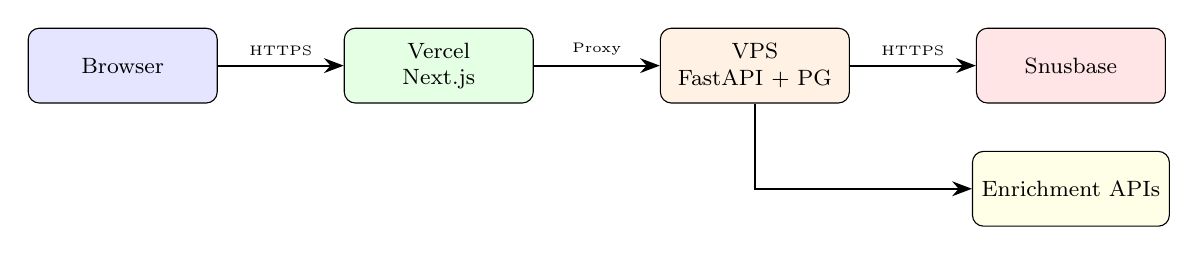
\begin{tikzpicture}[
  node distance=1.1cm and 1.6cm,
  box/.style={draw,rounded corners,minimum width=2.4cm,minimum height=0.95cm,
    align=center,font=\footnotesize},
  arrow/.style={-{Stealth[length=2.5mm]},thick},
]
  \node[box,fill=blue!10] (browser) {Browser};
  \node[box,fill=green!10,right=of browser] (vercel)
    {Vercel\\Next.js};
  \node[box,fill=orange!10,right=of vercel] (vps)
    {VPS\\FastAPI + PG};
  \node[box,fill=red!10,right=of vps] (snusbase) {Snusbase};
  \node[box,fill=yellow!10,below=0.6cm of snusbase] (freeapis)
    {Enrichment APIs};

  \draw[arrow] (browser) -- node[above,font=\tiny]{HTTPS} (vercel);
  \draw[arrow] (vercel) -- node[above,font=\tiny]{Proxy} (vps);
  \draw[arrow] (vps) -- node[above,font=\tiny]{HTTPS} (snusbase);
  \draw[arrow] (vps) |- (freeapis);
\end{tikzpicture}%
}
\caption{High-level system architecture.}
\label{fig:high-level-arch}
\end{figure}

% ----------------------------------------------------------------------------
\section*{Conclusion}

This first chapter established the project context, analyzed existing
OSINT platforms, and positioned the proposed solution as a practical,
security-conscious alternative for students and small security teams. The
next chapter details requirements and technology choices.

% ============================================================================
% Chapter II -- Requirements Analysis and Specification
% ============================================================================
\chapter{Requirements Analysis and Specification}
\label{chap:requirements}

\section*{Introduction}

This chapter defines the functional and technical foundations of the system:
actors, requirements, data model, and technology choices. These specifications
guide all design and implementation decisions in later chapters.

% ----------------------------------------------------------------------------
\section{Actor Identification}
\label{sec:actors}
% ----------------------------------------------------------------------------

The platform is a multi-user system built on role-based access control (RBAC).
Three actor levels interact with it:

\renewcommand{\arraystretch}{1.45}
\begin{table}[ht]
\centering
\caption{System actors and permissions.}
\label{tab:actors}
\begin{tabularx}{\textwidth}{@{} l X @{}}
\toprule
\textbf{Actor} & \textbf{Description and Permissions} \\
\midrule
Guest (unauthenticated) &
  Accesses public pages (landing, login, registration). May create an account
  only with a valid invite code. \\[8pt]
Analyst (default role) &
  Runs breach searches (7 types + wildcard), views credential results,
  consults search history, and re-runs past queries. \\[8pt]
Administrator &
  Inherits analyst permissions. Can manage user accounts and roles
  (planned extension). \\
\bottomrule
\end{tabularx}
\end{table}

Role enforcement is applied at the API layer through the \texttt{require\_role}
dependency. The \texttt{viewer} role is reserved for future use and is
explicitly excluded from search access.

\subsection{Use Case Diagram}
\label{sec:use-case}

\figref{fig:use-case} follows standard UML notation: actors outside the
system boundary, associations to use cases, and \texttt{<<include>>} /
\texttt{<<extend>>} relationships between use cases. Three roles interact
with the platform: unauthenticated guests (registration and login), analysts
(search and history), and administrators (user management).

\newpage
\thispagestyle{plain}
\vspace*{\fill}
\begin{center}
  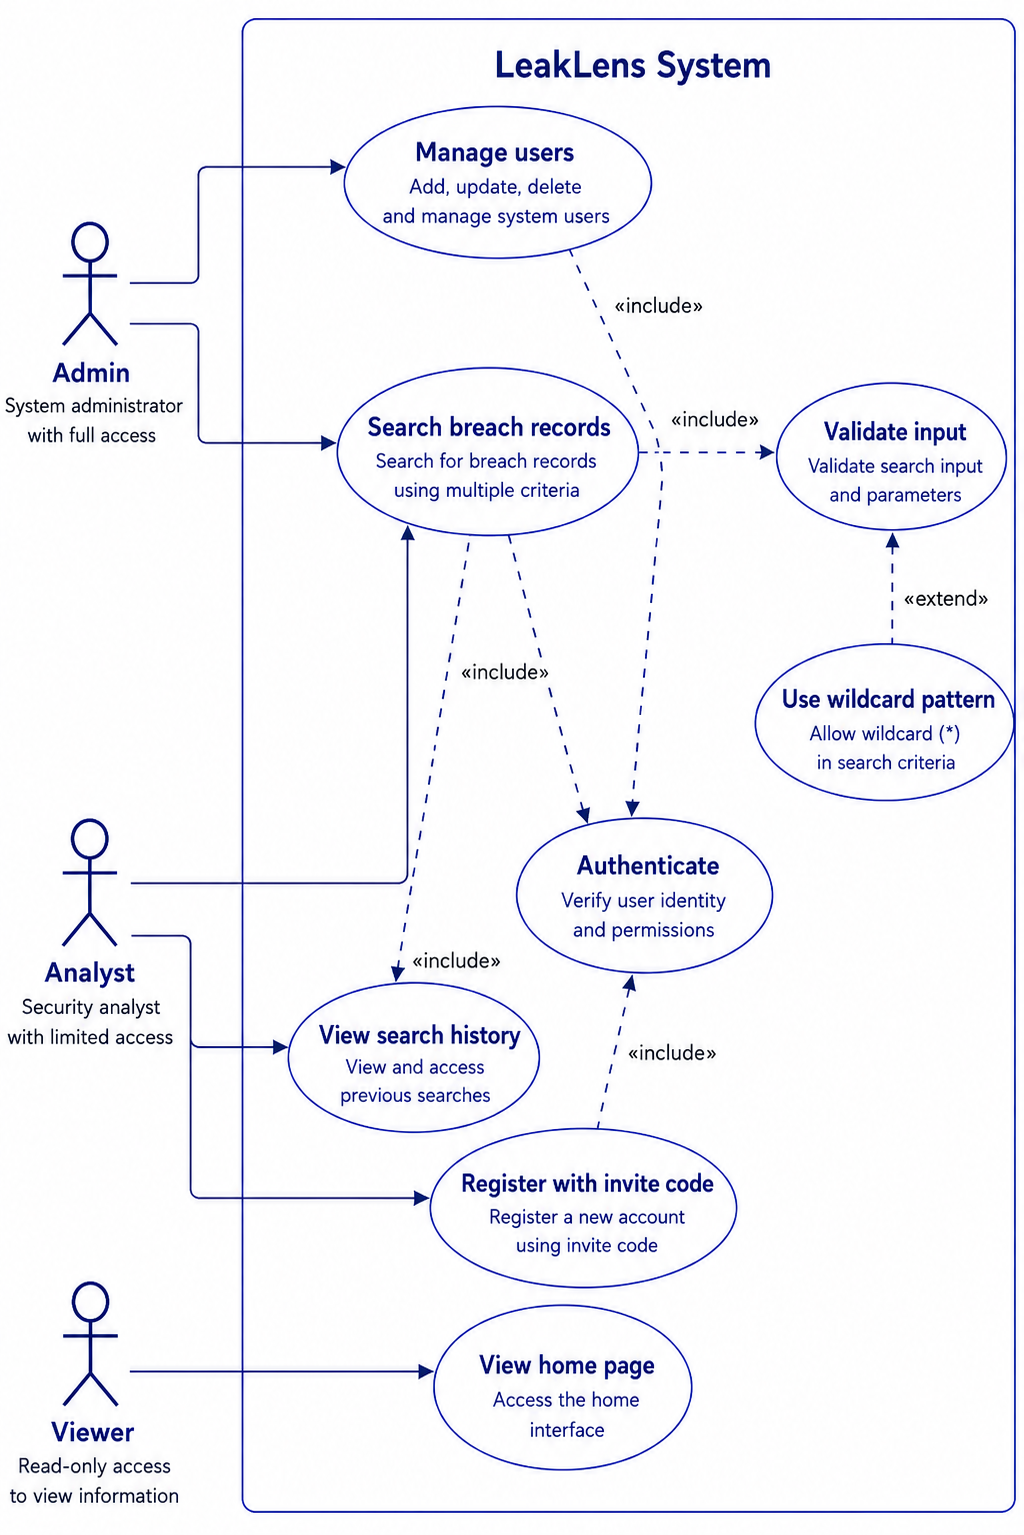
\includegraphics[
    width=\linewidth,
    height=0.82\textheight,
    keepaspectratio
  ]{usecase-diagram.png}
\end{center}
\vspace*{\fill}
\begin{center}
  \captionof{figure}{UML use case diagram.}
  \label{fig:use-case}
\end{center}
\vspace*{\fill}
\clearpage

\subsection{Breach Search Sequence}
\label{sec:search-sequence}

\figref{fig:search-sequence} describes the end-to-end path from user input
to displayed results. When an authenticated analyst submits a search, the
Next.js frontend sends a \texttt{POST /api/v1/search} request (proxied
server-side in production to avoid mixed-content issues). The FastAPI backend
validates the term against the selected search type, then delegates execution
to the \emph{Search Engine}, which queries Snusbase (\texttt{POST /data/search})
for breach records and calls free \emph{API Services} (LeakCheck, EmailRep,
Cert Spotter) for supplementary context. Results are scored by severity,
deduplicated, persisted as a \texttt{SearchQuery} row in PostgreSQL, and
returned to the client as a \texttt{SearchResponse} JSON payload.

\newpage
\thispagestyle{plain}
\vspace*{\fill}
\begin{center}
  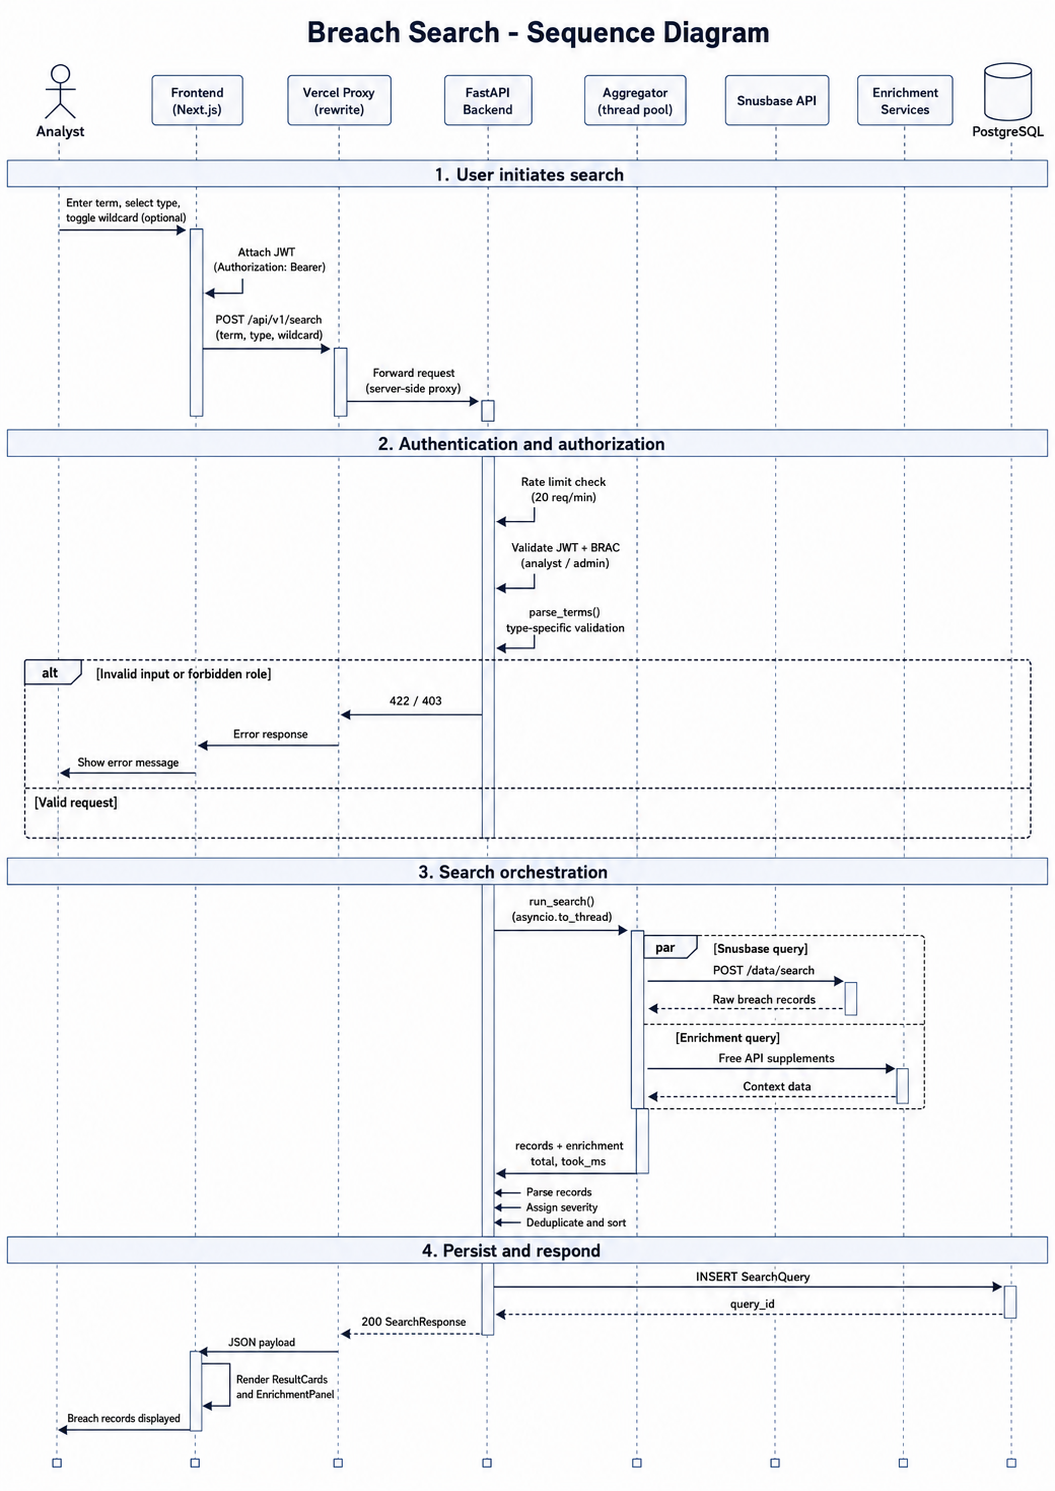
\includegraphics[
    width=\linewidth,
    height=0.82\textheight,
    keepaspectratio
  ]{search-sequence.png}
\end{center}
\vspace*{\fill}
\begin{center}
  \captionof{figure}{Breach search sequence diagram.}
  \label{fig:search-sequence}
\end{center}
\vspace*{\fill}

\clearpage

% ----------------------------------------------------------------------------
\section{Functional Requirements}
\label{sec:functional}
% ----------------------------------------------------------------------------

Functional requirements are grouped by domain.

\subsection{Authentication and Account Management}

\begin{description}[style=nextline,nosep,leftmargin=1.2cm]
  \item[FR-01] Create an account with email, full name, and password
    (minimum 12 characters, strength-validated). A valid invite code is
    required when the registration gate is active.
  \item[FR-02] Log in via email and password; receive JWT access and refresh
    tokens (access token expires after 15~minutes).
  \item[FR-03] Refresh an expired access token using the refresh token
    (valid for 7~days).
  \item[FR-04] Lock account after 5 failed login attempts for 15~minutes.
\end{description}

\subsection{Search}

\begin{description}[style=nextline,nosep,leftmargin=1.2cm]
  \item[FR-05] Search by seven types: email, username, IP, password, name,
    hash, or domain.
  \item[FR-06] Enforce type-specific input validation (email regex, IP
    format, hash patterns).
  \item[FR-07] Wildcard mode for pattern matching (e.g.,
    \texttt{\%@gmail.com}); minimum 3 characters.
  \item[FR-08] Display results grouped by source database with severity
    ratings (critical / high / medium / low).
\end{description}

\subsection{Enrichment}

\begin{description}[style=nextline,nosep,leftmargin=1.2cm]
  \item[FR-09] Email searches: LeakCheck (breach names) and EmailRep.io
    (reputation score).
  \item[FR-10] Domain searches: Cert Spotter (subdomains) and Snusbase WHOIS.
  \item[FR-11] IP searches: Snusbase IP WHOIS lookup.
\end{description}

\subsection{Search History and Authorization}

\begin{description}[style=nextline,nosep,leftmargin=1.2cm]
  \item[FR-12] Record every search (query, type, result count, timestamp).
  \item[FR-13] View the last 200 searches and re-run any query.
  \item[FR-14] Restrict search to \texttt{analyst} and \texttt{admin} roles;
    \texttt{viewer} is read-only on history.
\end{description}

% ----------------------------------------------------------------------------
\section{Non-Functional Requirements}
\label{sec:nonfunctional}
% ----------------------------------------------------------------------------

\renewcommand{\arraystretch}{1.45}
\begin{table}[ht]
\centering
\caption{Non-functional requirements.}
\label{tab:nfr}
\small
\begin{tabularx}{\textwidth}{@{} l L{3.5cm} X @{}}
\toprule
\textbf{Category} & \textbf{Requirement} & \textbf{Solution} \\
\midrule
Security &
  Protect data in transit and at rest &
  JWT (access + refresh), bcrypt (12 rounds), rate limiting, CSP, HSTS,
  CORS, invite-code gating, constant-time login \\[8pt]
Performance &
  Search response $<$ 3\,s &
  \texttt{ThreadPoolExecutor} for concurrent API calls; async SQLAlchemy
  for database I/O \\[8pt]
Availability &
  Auto-recovery after failure &
  Docker \texttt{restart: unless-stopped}; PostgreSQL and backend health
  checks \\[8pt]
Portability &
  Same behaviour in dev and prod &
  Alpine multi-stage Docker build; \texttt{docker-compose.yml} \\[8pt]
Maintainability &
  Simple frontend updates &
  Vercel auto-deploy on \texttt{git push} \\[8pt]
Compliance &
  Responsible breach-data use &
  Invite-only registration; no local credential storage; rate limits \\
\bottomrule
\end{tabularx}
\end{table}

% ----------------------------------------------------------------------------
\section{Data Model}
\label{sec:datamodel}
% ----------------------------------------------------------------------------

The data model uses SQLAlchemy (async) with PostgreSQL~16. Two core entities
and two enumerations structure persistence.

\subsection{Enumerations}

\begin{itemize}[nosep]
  \item \textbf{UserRole:} \texttt{admin}, \texttt{analyst}, \texttt{viewer}
  \item \textbf{SearchType:} \texttt{email}, \texttt{username}, \texttt{ip},
        \texttt{password}, \texttt{hash}, \texttt{name}, \texttt{domain}
\end{itemize}

\subsection{Relationships and Integrity}

\begin{itemize}[nosep]
  \item A \texttt{User} owns zero or more \texttt{SearchQuery} records
        (one-to-many).
  \item Deleting a \texttt{User} cascades to their \texttt{SearchQuery}
        records (\texttt{onDelete: CASCADE}).
  \item The \texttt{email} field on \texttt{User} is unique.
  \item Passwords are stored as bcrypt hashes; plaintext is never persisted.
\end{itemize}

\begin{figure}[ht]
\centering
\tikzfig{%
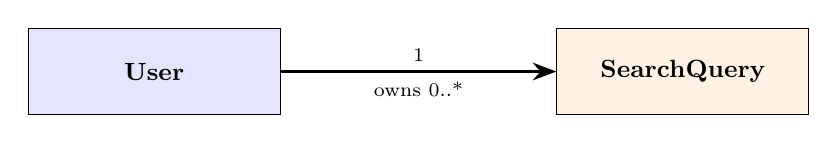
\begin{tikzpicture}[
  entity/.style={draw,rectangle,minimum width=3.2cm,minimum height=1.1cm,
    align=center,font=\small\bfseries},
  arrow/.style={-{Stealth[length=3mm]},thick},
]
  \node[entity,fill=blue!10] (user) {User};
  \node[entity,fill=orange!10,right=3.5cm of user] (query) {SearchQuery};
  \draw[arrow] (user) -- node[above,font=\scriptsize]{1}
    node[below,font=\scriptsize]{owns 0..*} (query);
\end{tikzpicture}%
}
\caption{Entity-relationship diagram.}
\label{fig:erd}
\end{figure}

% ----------------------------------------------------------------------------
\section{Technology Choices}
\label{sec:techstack}
% ----------------------------------------------------------------------------

Table~\ref{tab:appstack} lists the development stack; Table~\ref{tab:infra}
covers deployment and operations.

\renewcommand{\arraystretch}{1.55}
\begin{table}[H]
\centering
\caption{Application stack --- development technologies.}
\label{tab:appstack}
\small
\begin{tabularx}{\textwidth}{@{} c l l X @{}}
\toprule
\textbf{Logo} & \textbf{Technology} & \textbf{Role} & \textbf{Justification} \\
\midrule
\logobox{0.55cm}{nextjs-logo.png} &
  Next.js~15 & Frontend &
  React framework with App Router, SSR, and API rewrites for backend
  proxying. \\[6pt]
\logobox{0.55cm}{fastapi-logo.png} &
  FastAPI & Backend API &
  Async Python framework with Pydantic validation and dependency injection
  for RBAC. \\[6pt]
\logobox{0.55cm}{postgresql-logo.png} &
  PostgreSQL~16 & Database &
  RDBMS with UUID support and async driver (\texttt{asyncpg}) via
  SQLAlchemy. \\[6pt]
\logobox{0.55cm}{snusbase-logo.png} &
  Snusbase API & Breach engine &
  Primary data source: 7 search types, wildcard, WHOIS lookups. \\[6pt]
 &
  SQLAlchemy & ORM &
  Async session support and declarative models. \\[6pt]
 &
  httpx & HTTP client &
  External API calls (Snusbase, enrichment services). \\[6pt]
 &
  Zustand & Client state &
  Lightweight JWT and auth state on the frontend. \\
\bottomrule
\end{tabularx}
\end{table}

\renewcommand{\arraystretch}{1.45}
\begin{table}[H]
\centering
\caption{Infrastructure --- deployment and operations.}
\label{tab:infra}
\small
\begin{tabularx}{\textwidth}{@{} l l X @{}}
\toprule
\textbf{Technology} & \textbf{Role} & \textbf{Justification} \\
\midrule
Docker (Alpine) & Containerization &
  Multi-stage build, non-root user, resource limits, Trivy scanning. \\[6pt]
Docker Compose & Orchestration &
  Backend + PostgreSQL stack with health checks and network isolation. \\[6pt]
Vercel & Frontend hosting &
  Automatic HTTPS, CDN, git-push deploy. \\[6pt]
VPS (Linux) & Backend hosting &
  Dedicated server running Docker Compose. \\[6pt]
Nginx Proxy Manager & Reverse proxy &
  TLS termination and subdomain routing (multi-project VPS). \\[6pt]
GitHub & Version control &
  Source hosting; Vercel deploy triggered on \texttt{main} push. \\
\bottomrule
\end{tabularx}
\end{table}

\FloatBarrier

% ----------------------------------------------------------------------------
\section*{Conclusion}

This chapter defined 14 functional requirements, 6 non-functional categories,
a two-entity data model, and the technology stack. These specifications form
the basis for the architecture design in the next chapter.

% ============================================================================
% Chapter III -- Architecture Design and Security
% ============================================================================
\chapter{Architecture Design and Security}
\label{chap:architecture}

\section*{Introduction}

This chapter presents the system architecture and security design in detail,
from global topology down to individual controls.

% ----------------------------------------------------------------------------
\section{Global System Architecture}
\label{sec:global-arch}
% ----------------------------------------------------------------------------

The system follows a split-deployment model with clear separation between
frontend delivery and backend processing. \figref{fig:global-arch} summarizes
the production topology end to end: the \textbf{Browser} connects to the
\textbf{Frontend Layer (Vercel)} over HTTPS, where \textbf{Next.js~15} serves
the UI and proxies API traffic server-side; requests reach the \textbf{VPS},
where \textbf{Nginx Proxy Manager} terminates inbound connections and forwards
them into a \textbf{Docker Compose} stack running \textbf{FastAPI} and
\textbf{PostgreSQL~16}; the backend then queries \textbf{Snusbase} and free
\textbf{Enrichment APIs} (LeakCheck, EmailRep.io, Cert Spotter) over HTTPS.
No breach credentials are persisted locally---only user accounts and search
metadata are stored in PostgreSQL.

\begin{figure}[H]
\centering
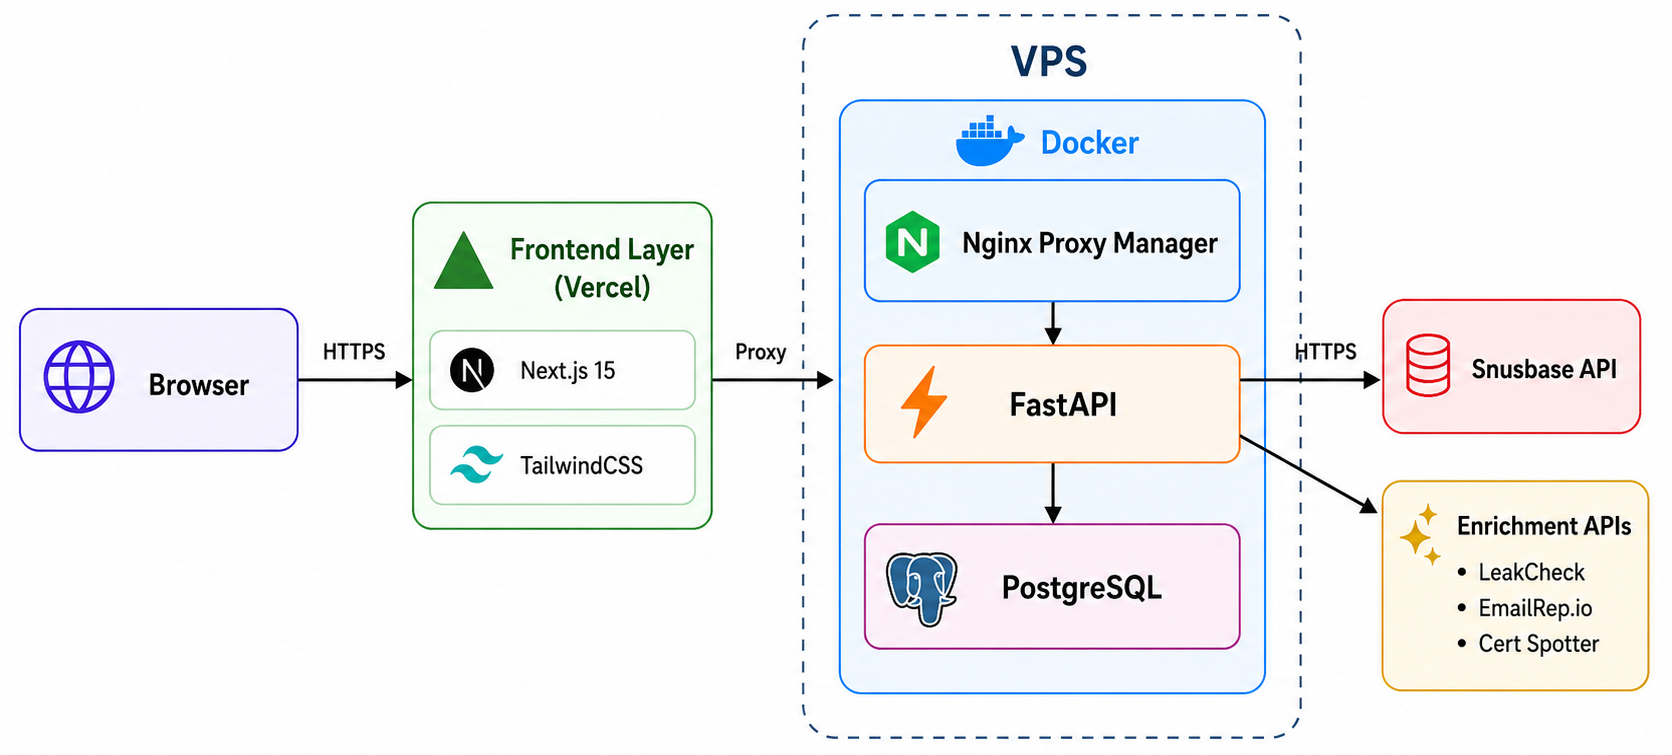
\includegraphics[
  width=\linewidth,
  keepaspectratio
]{architecture-diag.png}
\caption{Global system architecture.}
\label{fig:global-arch}
\end{figure}

\textbf{Key architectural decisions:}

\begin{enumerate}[nosep]
  \item \textbf{Split deployment:} The frontend is hosted on Vercel (automatic
        HTTPS, global CDN), while the backend runs on a dedicated VPS. This
        separates static asset delivery from API processing and database I/O.
  \item \textbf{Rewrite proxy pattern:} In production, Next.js rewrites all
        \texttt{/api/v1/*} requests to the backend server-side. The browser
        never makes a direct cross-origin HTTP call, eliminating mixed-content
        issues when the API is exposed on plain HTTP behind the VPS.
  \item \textbf{Docker containerization:} The VPS backend is orchestrated with
        \texttt{docker-compose.yml}: a \textbf{PostgreSQL} container on an
        internal bridge network and a \textbf{FastAPI} container built from a
        multi-stage Alpine Dockerfile (non-root user, health checks, CPU/memory
        limits, \texttt{no-new-privileges}). The database is not reachable from
        the public internet.
  \item \textbf{Nginx Proxy Manager:} On the VPS, Nginx Proxy Manager sits in
        front of the Docker stack as the reverse proxy entry point. It routes
        incoming API traffic to the backend container, supports TLS termination
        when a custom subdomain is configured, and coexists with other projects
        on the same host through hostname-based routing.
  \item \textbf{Stateless backend:} FastAPI stores no server-side sessions.
        Authentication state is carried entirely in JWT access and refresh
        tokens, which simplifies scaling and container restarts.
  \item \textbf{External data sources:} Breach records are fetched in real
        time from Snusbase and enrichment APIs; only search audit metadata
        (query, type, result count, timestamp) is written to PostgreSQL.
\end{enumerate}

% ----------------------------------------------------------------------------
\section{Backend API Design}
\label{sec:api-design}
% ----------------------------------------------------------------------------

The backend exposes a RESTful API under the \texttt{/api/v1} prefix. All
endpoints return JSON and follow consistent error formats.

\begin{table}[ht]
\centering
\caption{REST API endpoints.}
\label{tab:endpoints}
\small
\begin{tabularx}{\textwidth}{@{} l l l X @{}}
\toprule
\textbf{Method} & \textbf{Endpoint} & \textbf{Auth} & \textbf{Description} \\
\midrule
POST & \texttt{/auth/register} & None &
  Create account (email, password, invite code) \\
POST & \texttt{/auth/login} & None &
  Authenticate; returns access + refresh tokens \\
POST & \texttt{/auth/refresh} & None &
  Exchange refresh token for new access token \\
GET  & \texttt{/auth/me} & Bearer &
  Return current user profile \\
POST & \texttt{/search} & Analyst+ &
  Search leaked databases (7 types + wildcard) \\
GET  & \texttt{/history} & Bearer &
  Return user's last 200 searches \\
GET  & \texttt{/health} & None &
  Health check (returns \texttt{\{status: ok\}}) \\
\bottomrule
\end{tabularx}
\end{table}

Each protected endpoint uses FastAPI's dependency injection system. The
\texttt{CurrentUser} dependency extracts and validates the JWT from the
\texttt{Authorization} header. The \texttt{SearchUser} dependency
additionally enforces role requirements via \texttt{require\_role(ANALYST,
ADMIN)}.

% ----------------------------------------------------------------------------
\section{Search Engine Pipeline}
\label{sec:search-pipeline}
% ----------------------------------------------------------------------------

The search pipeline orchestrates validation, API calls, enrichment, and
result aggregation concurrently. \figref{fig:search-pipeline} shows how a
query flows from the API layer through the Search Engine to Snusbase and
supplementary API Services before results are scored, deduplicated, and
returned.

\begin{figure}[H]
\centering
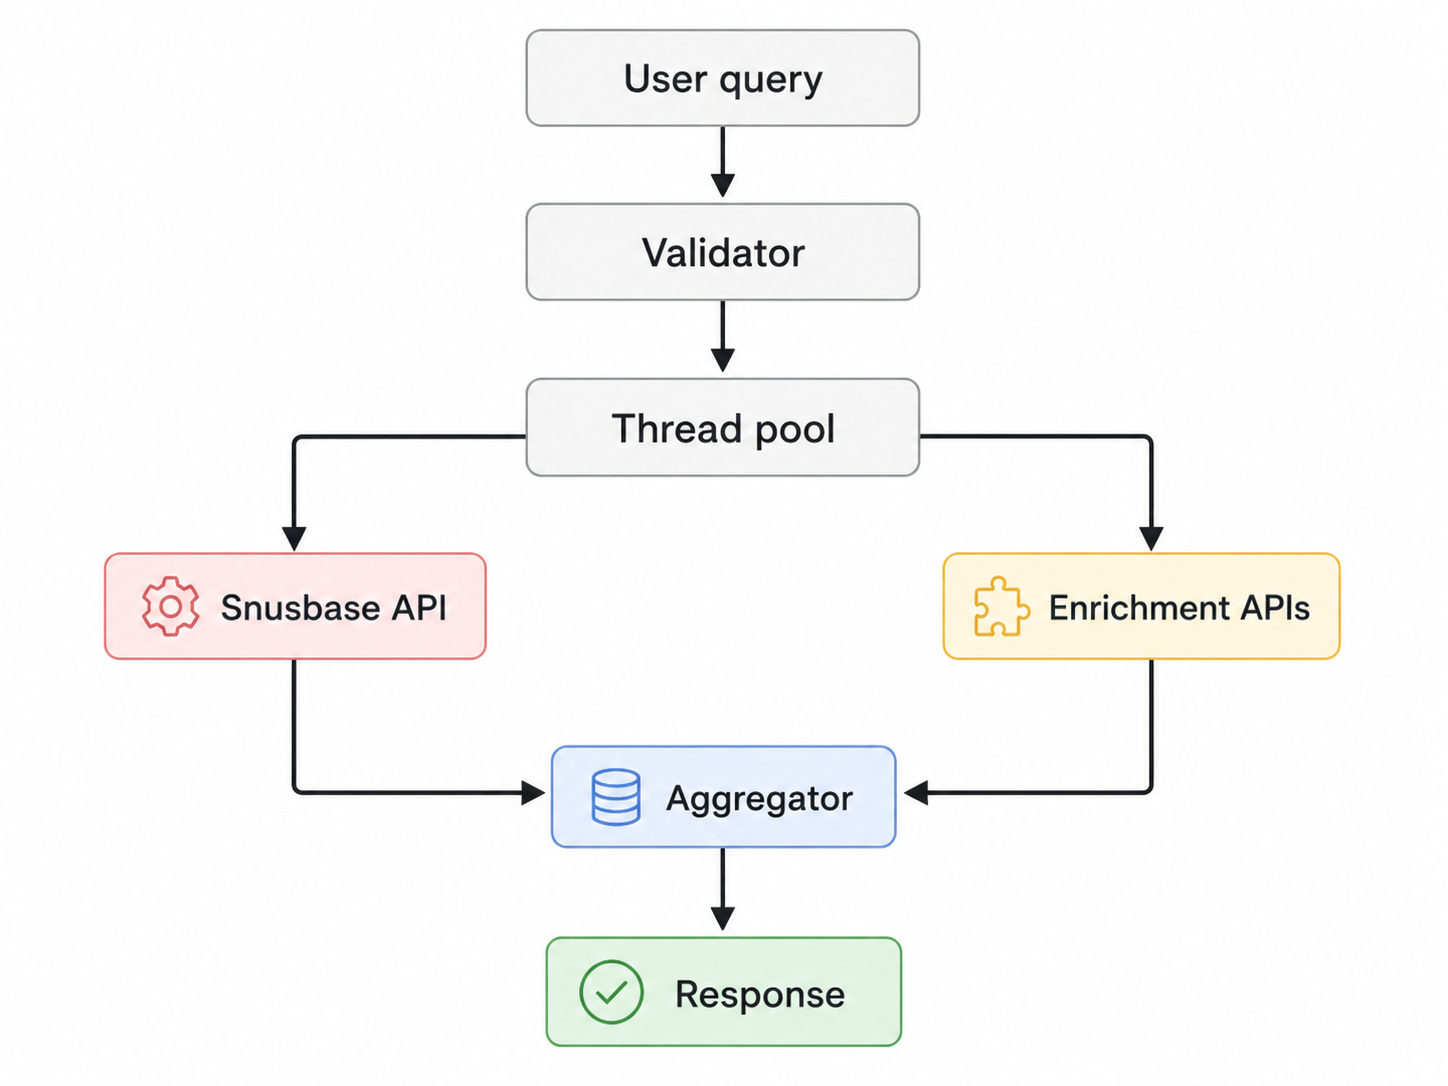
\includegraphics[
  width=\linewidth,
  keepaspectratio
]{search-diag.png}
\caption{Search engine pipeline.}
\label{fig:search-pipeline}
\end{figure}

\subsection{Input Validation}

The \texttt{validators} module enforces type-specific rules:

\begin{itemize}[nosep]
  \item \textbf{Email:} Must match a standard email regex.
  \item \textbf{Domain:} Must be a valid domain extracted via
        \texttt{tldextract}.
  \item \textbf{IP:} Validated against IPv4/IPv6 format.
  \item \textbf{Hash:} Must match MD5 (32~hex), SHA-1 (40~hex), or
        SHA-256 (64~hex) patterns.
  \item \textbf{Username/Name/Password:} Minimum 2 characters, maximum 320.
  \item \textbf{Wildcard mode:} Relaxes all format checks but enforces a
        3-character minimum to prevent overly broad queries.
\end{itemize}

\subsection{Concurrent Execution}

The aggregator uses a \texttt{ThreadPoolExecutor} with 4 workers to run the
Snusbase API call and enrichment calls in parallel. Since the Snusbase client
(\texttt{httpx}) uses synchronous HTTP, \texttt{asyncio.to\_thread} is not
needed---the executor offloads blocking I/O from the event loop naturally.

\subsection{Severity Scoring}

Each leak record is assigned a severity level based on the fields present:

\begin{itemize}[nosep]
  \item \textbf{Critical:} Password in plaintext or cracked hash present.
  \item \textbf{High:} Hash present (but no plaintext password).
  \item \textbf{Medium:} Email and username exposed, but no credentials.
  \item \textbf{Low:} Minimal exposure (e.g., only an email address).
\end{itemize}

% ----------------------------------------------------------------------------
\section{Security Architecture}
\label{sec:security}
% ----------------------------------------------------------------------------

This section details nine security layers forming a defense-in-depth strategy
aligned with OWASP best practices~\cite{owasp-top10}.

\subsection{Authentication: JWT Access and Refresh Tokens}

Authentication uses a dual-token scheme:

\begin{itemize}[nosep]
  \item \textbf{Access token:} Short-lived (15~minutes), signed with
        HS256 using a 256-bit secret. Contains the user ID and role in its
        claims. Sent in the \texttt{Authorization: Bearer} header.
  \item \textbf{Refresh token:} Longer-lived (7~days), used exclusively to
        obtain a new access token. Transmitted in the request body, never
        stored in cookies.
\end{itemize}

Password hashing uses \texttt{bcrypt} with 12 rounds (configurable via
\texttt{BCRYPT\_ROUNDS}), producing a 60-character hash that includes the
salt.

\begin{lstlisting}[language=Python,caption={JWT token creation (simplified).}]
def create_access_token(sub: str, extra_claims: dict) -> str:
    payload = {
        "sub": sub,
        "type": "access",
        "exp": datetime.utcnow()
              + timedelta(minutes=settings.ACCESS_TOKEN_EXPIRE_MINUTES),
        **extra_claims,  # includes {"role": "analyst"}
    }
    return jwt.encode(payload, settings.SECRET_KEY,
                      algorithm=settings.ALGORITHM)
\end{lstlisting}

\subsection{Authorization: Role-Based Access Control (RBAC)}

Access control is enforced at the API layer through FastAPI's dependency
injection:

\begin{lstlisting}[language=Python,caption={RBAC dependency injection.}]
def require_role(*roles: UserRole):
    def checker(user: User = Depends(get_current_active_user)):
        if user.role not in roles:
            raise HTTPException(403, "Insufficient permissions")
        return user
    return checker

# Applied to the search endpoint:
SearchUser = Annotated[User,
    Depends(require_role(UserRole.ANALYST, UserRole.ADMIN))]
\end{lstlisting}

Three roles are defined: \texttt{admin} (full access), \texttt{analyst}
(search + history), and \texttt{viewer} (history only, no search).

\subsection{Anti-Enumeration: Constant-Time Login}

A common attack vector is \emph{timing-based user enumeration}: an attacker
measures login response times to determine whether an email exists in the
system (bcrypt verification takes measurable time; skipping it is fast).

The system mitigates timing-based user enumeration by running a dummy bcrypt
verification when the account is not found:

\begin{lstlisting}[language=Python,caption={Constant-time login defense.}]
_DUMMY_HASH = hash_password("dummy-password-for-constant-time")

if user is None:
    verify_password(form_data.password, _DUMMY_HASH)  # same timing
    raise auth_error
\end{lstlisting}

Combined with the generic error message ``Incorrect email or password,'' this
makes it infeasible to distinguish between a non-existent account and a wrong
password.

\subsection{Registration Gate: Invite Code}

To prevent unauthorized sign-ups, registration requires a matching invite
code when \texttt{INVITE\_CODE} is configured:

\begin{lstlisting}[language=Python,caption={Invite-code verification with constant-time comparison.}]
if settings.INVITE_CODE:
    if not hmac.compare_digest(provided, settings.INVITE_CODE):
        raise HTTPException(403,
            "A valid invite code is required to register.")
\end{lstlisting}

The use of \texttt{hmac.compare\_digest} prevents timing attacks on the
invite code itself. The registration error for duplicate emails is also
generic (``Unable to register with the provided details'') to avoid
confirming which emails are already registered.

\subsection{Rate Limiting}

Per-endpoint rate limiting is implemented using \texttt{slowapi} (a
Starlette/FastAPI wrapper around \texttt{limits}):

\begin{table}[ht]
\centering
\caption{Rate limits per endpoint category.}
\label{tab:rate-limits}
\begin{tabular}{@{} l c @{}}
\toprule
\textbf{Endpoint category} & \textbf{Limit (per minute)} \\
\midrule
Authentication (\texttt{/auth/*}) & 5 \\
Search (\texttt{/search})         & 20 \\
General API                       & 60 \\
\bottomrule
\end{tabular}
\end{table}

Rate limits are keyed by client IP. When exceeded, the API returns
\texttt{429 Too Many Requests} with a \texttt{Retry-After} header.

\subsection{HTTP Security Headers}

The backend injects strict security headers on every response via a custom
middleware (\texttt{SecurityHeadersMiddleware}):

\begin{table}[ht]
\centering
\caption{HTTP security headers.}
\label{tab:headers}
\small
\begin{tabularx}{\textwidth}{@{} l X @{}}
\toprule
\textbf{Header} & \textbf{Value and Purpose} \\
\midrule
\texttt{X-Content-Type-Options} &
  \texttt{nosniff} --- prevents MIME-type sniffing attacks \\
\texttt{X-Frame-Options} &
  \texttt{DENY} --- blocks clickjacking via iframes \\
\texttt{Referrer-Policy} &
  \texttt{strict-origin-when-cross-origin} --- limits referrer leakage \\
\texttt{Permissions-Policy} &
  Disables geolocation, microphone, camera, payment, USB \\
\texttt{Cross-Origin-Opener-Policy} &
  \texttt{same-origin} --- isolates browsing context \\
\texttt{Strict-Transport-Security} &
  \texttt{max-age=63072000; includeSubDomains; preload} (production only) \\
\bottomrule
\end{tabularx}
\end{table}

The frontend additionally sets a \textbf{Content Security Policy (CSP)} via
\texttt{next.config.js}, restricting script sources, connection targets, and
frame ancestors.

\subsection{CORS: Strict Origin Allowlist}

Cross-Origin Resource Sharing is configured with an explicit allowlist of
origins (set via the \texttt{CORS\_ORIGINS} environment variable). In
production, only the Vercel frontend domain is permitted. Credentials
(\texttt{allow\_credentials=True}) and specific HTTP methods are explicitly
listed. Wildcard origins (\texttt{*}) are never used.

\subsection{Input Validation}

All user input passes through Pydantic models (FastAPI's built-in validation
layer) before reaching business logic:

\begin{itemize}[nosep]
  \item Email fields validated by \texttt{pydantic[email-validator]}.
  \item Password: minimum 12 characters, strength-checked (uppercase,
        lowercase, digit, special character).
  \item Search terms: type-specific regex, maximum 25 terms per query,
        320-character limit per term.
  \item Invite code: maximum 128 characters.
\end{itemize}

\subsection{Docker Security}

The containerization strategy follows Docker security best practices:

\begin{enumerate}[nosep]
  \item \textbf{Alpine base image:} Minimal attack surface (5~MB base vs.
        120~MB for Debian).
  \item \textbf{Multi-stage build:} Build dependencies (compilers, headers)
        are excluded from the production image.
  \item \textbf{Non-root execution:} The application runs as user
        \texttt{leaklens} (UID~1000), never as root.
  \item \textbf{\texttt{no-new-privileges}:} The Docker security option
        prevents privilege escalation inside the container.
  \item \textbf{\texttt{forwarded-allow-ips}:} Uvicorn trusts
        \texttt{X-Forwarded-*} headers only from the Docker bridge network
        (\texttt{127.0.0.1,172.16.0.0/12}), preventing IP spoofing from
        external clients.
  \item \textbf{\texttt{.dockerignore}:} Excludes \texttt{.env}, tests, and
        Python cache from the build context.
  \item \textbf{Resource limits:} Docker Compose enforces CPU and memory
        limits (1.5~CPU / 512~MB for backend, 1.0~CPU / 512~MB for
        PostgreSQL).
  \item \textbf{Trivy scanning:} A \texttt{trivy-scan.sh} script builds the
        image and scans it for known vulnerabilities before deployment.
\end{enumerate}

\begin{lstlisting}[language={},caption={Dockerfile excerpt --- non-root user and restricted forwarding.},label={lst:dockerfile}]
# Runtime stage
FROM python:3.12-alpine AS runtime
RUN adduser -D -u 1000 leaklens
COPY --from=builder /install /usr/local
COPY ./app /home/leaklens/app
USER leaklens
CMD ["uvicorn", "app.main:app", "--host", "0.0.0.0", "--port", "8000", \
     "--proxy-headers", "--forwarded-allow-ips=127.0.0.1,172.16.0.0/12"]
\end{lstlisting}

% ----------------------------------------------------------------------------
\section{Containerization with Docker}
\label{sec:docker}
% ----------------------------------------------------------------------------

The backend Dockerfile uses a two-stage build strategy:

\begin{figure}[ht]
\centering
\tikzfig{%
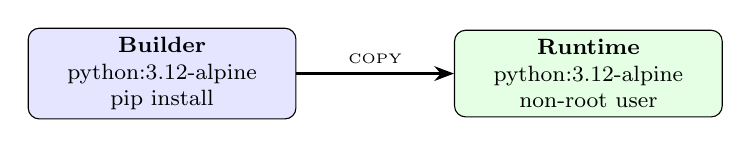
\begin{tikzpicture}[
  stage/.style={draw,rounded corners,minimum width=3.4cm,minimum height=1.1cm,
    align=center,font=\footnotesize},
  arrow/.style={-{Stealth[length=2.5mm]},thick},
]
  \node[stage,fill=blue!10] (builder) {\textbf{Builder}\\python:3.12-alpine\\pip install};
  \node[stage,fill=green!10,right=2cm of builder] (runtime)
    {\textbf{Runtime}\\python:3.12-alpine\\non-root user};
  \draw[arrow] (builder) -- node[above,font=\tiny]{COPY} (runtime);
\end{tikzpicture}%
}
\caption{Docker multi-stage build.}
\label{fig:docker-stages}
\end{figure}

The builder stage installs all Python dependencies (including C extensions
like \texttt{bcrypt} and \texttt{asyncpg}) with their build-time headers. The
runtime stage copies only the compiled packages, resulting in a lean
production image.

% ----------------------------------------------------------------------------
\section{Deployment Architecture}
\label{sec:deployment}
% ----------------------------------------------------------------------------

\begin{figure}[ht]
\centering
\tikzfig{%
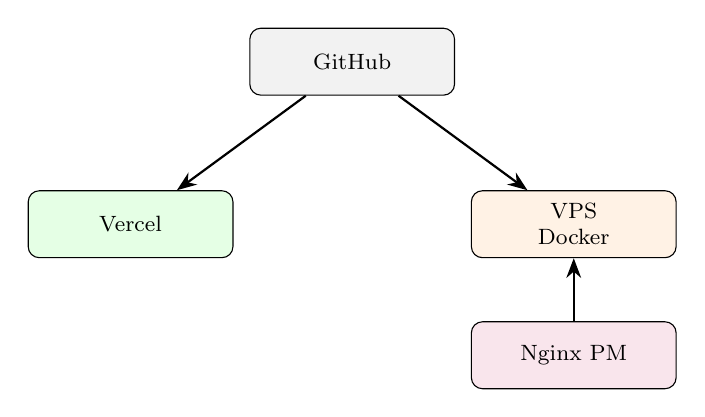
\begin{tikzpicture}[
  node distance=0.9cm and 1.5cm,
  box/.style={draw,rounded corners,minimum width=2.6cm,minimum height=0.85cm,
    align=center,font=\footnotesize},
  arrow/.style={-{Stealth[length=2.5mm]},thick},
]
  \node[box,fill=gray!10] (github) {GitHub};
  \node[box,fill=green!10,below left=1.2cm and 0.2cm of github] (vercel)
    {Vercel};
  \node[box,fill=orange!10,below right=1.2cm and 0.2cm of github] (vps)
    {VPS\\Docker};
  \node[box,fill=purple!10,below=0.8cm of vps] (npm) {Nginx PM};
  \draw[arrow] (github) -- (vercel);
  \draw[arrow] (github) -- (vps);
  \draw[arrow] (npm) -- (vps);
\end{tikzpicture}%
}
\caption{Deployment workflow.}
\label{fig:deployment}
\end{figure}

\begin{itemize}[nosep]
  \item \textbf{Frontend (Vercel):} Every push to \texttt{main} triggers an
        automatic build and deployment. Vercel provides HTTPS, a global CDN,
        and preview deployments for pull requests.
  \item \textbf{Backend (VPS):} The operator SSHs into the VPS, pulls the
        latest code, and runs \texttt{docker compose up -d -{}-build}. The
        PostgreSQL data is persisted on a named Docker volume.
  \item \textbf{Nginx Proxy Manager:} Already present on the VPS for other
        projects, it routes traffic by subdomain with automatic Let's Encrypt
        certificates. The VPS can host multiple projects simultaneously, each
        with its own subdomain.
  \item \textbf{Environment variables:} Production secrets (\texttt{SECRET\_KEY},
        \texttt{POSTGRES\_PASSWORD}, \texttt{SNUSBASE\_API\_KEY},
        \texttt{INVITE\_CODE}) are stored in a \texttt{.env} file on the VPS,
        never committed to Git. A \texttt{.env.example} template is provided
        in the repository.
\end{itemize}

% ----------------------------------------------------------------------------
\section*{Conclusion}

This chapter presented the system architecture and its nine security layers.
The search pipeline handles concurrent API orchestration with input validation
and severity scoring. The next chapter shows the concrete realization through
screenshots and production metrics.

% ============================================================================
% Chapter IV -- Implementation and Results
% ============================================================================
\chapter{Implementation and Results}
\label{chap:implementation}

\section*{Introduction}

This chapter presents the concrete realization through screenshots, deployment
evidence, and live search demonstrations on the production instance at
\url{https://leakslens.vercel.app}.

% ----------------------------------------------------------------------------
\section{Development Environment}
\label{sec:devenv}
% ----------------------------------------------------------------------------

\begin{table}[H]
\centering
\caption{Development and production environment.}
\label{tab:devenv}
\small
\begin{tabularx}{\textwidth}{@{} l l X @{}}
\toprule
\textbf{Component} & \textbf{Version / Ref.} & \textbf{Usage} \\
\midrule
Development OS    & Windows 11              & Local development and testing \\
Python            & 3.12 (Alpine)           & Backend runtime \\
Node.js           & 20 LTS                  & Frontend build and SSR \\
Docker Desktop    & 27+                     & Local containerization \\
Cursor IDE        & Latest                  & Code editor with AI assistance \\
Git               & 2.x                     & Version control \\
VPS OS            & Ubuntu 22.04 LTS        & Production server \\
VPS Specs         & 91.148.168.36           & Dedicated server \\
Docker (VPS)      & 24+                     & Production containers \\
Nginx Proxy Mgr   & Latest                  & Reverse proxy with SSL \\
Vercel            & Free tier               & Frontend hosting \\
\bottomrule
\end{tabularx}
\end{table}

% ----------------------------------------------------------------------------
\section{User Interface}
\label{sec:ui}
% ----------------------------------------------------------------------------

The frontend uses Next.js~15, Tailwind CSS, and shadcn/ui with a dark theme
suited to extended research sessions.

\subsection{Landing Page (Guest View)}

The landing page presents \leaklens{} to unauthenticated visitors. It
displays the platform's purpose, key features (billions of records, full
credentials, 7 search types, enrichment), and call-to-action buttons for
signing in or creating an account.

\begin{figure}[H]
\centering
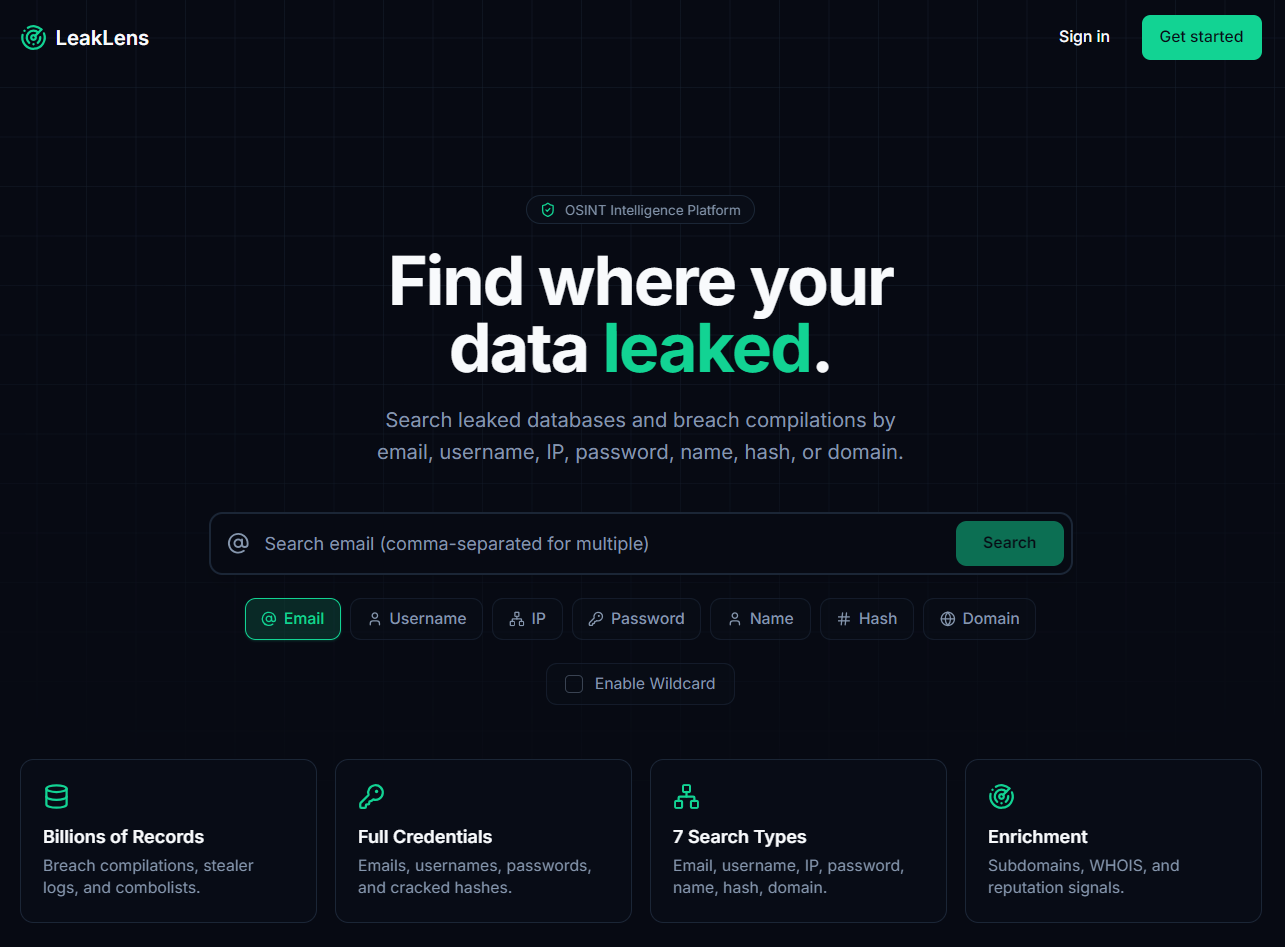
\includegraphics[width=\linewidth,keepaspectratio]{landing-guest.png}
\caption{Landing page of \leaklens{} (\url{https://leakslens.vercel.app}).}
\label{fig:landing}
\end{figure}

\subsection{Registration and Login}

Account creation requires email, full name, password, and a valid invite code
when the registration gate is active. The login form accepts email and password;
after successful authentication, the user is redirected to the search
interface. \figref{fig:register} and \figref{fig:login} show both forms on
the same page layout.

\begin{figure}[H]
\centering
\begin{minipage}[t]{0.47\linewidth}
  \centering
  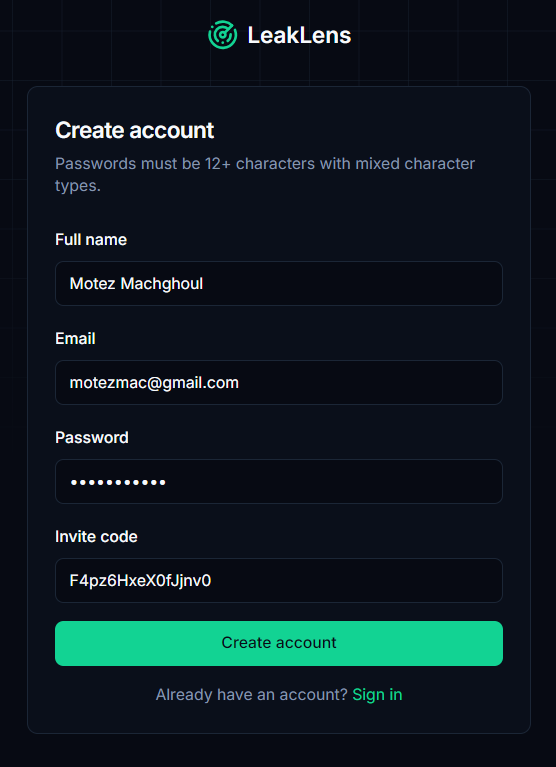
\includegraphics[width=\linewidth,keepaspectratio]{register.png}\\[4pt]
  \captionof{figure}{Registration form with invite-code gate.}
  \label{fig:register}
\end{minipage}\hfill
\begin{minipage}[t]{0.47\linewidth}
  \centering
  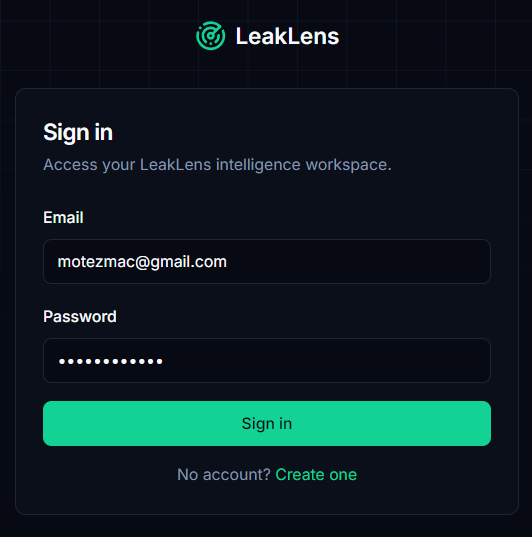
\includegraphics[width=\linewidth,keepaspectratio]{login.png}\\[4pt]
  \captionof{figure}{Login form.}
  \label{fig:login}
\end{minipage}
\end{figure}

\subsection{Home Page (Authenticated View)}

Once logged in, the user sees a streamlined home page with the search bar
prominently displayed. Seven search-type chips (Email, Username, IP,
Password, Name, Hash, Domain) allow quick type selection, and a wildcard
toggle enables pattern matching.

\begin{figure}[H]
\centering
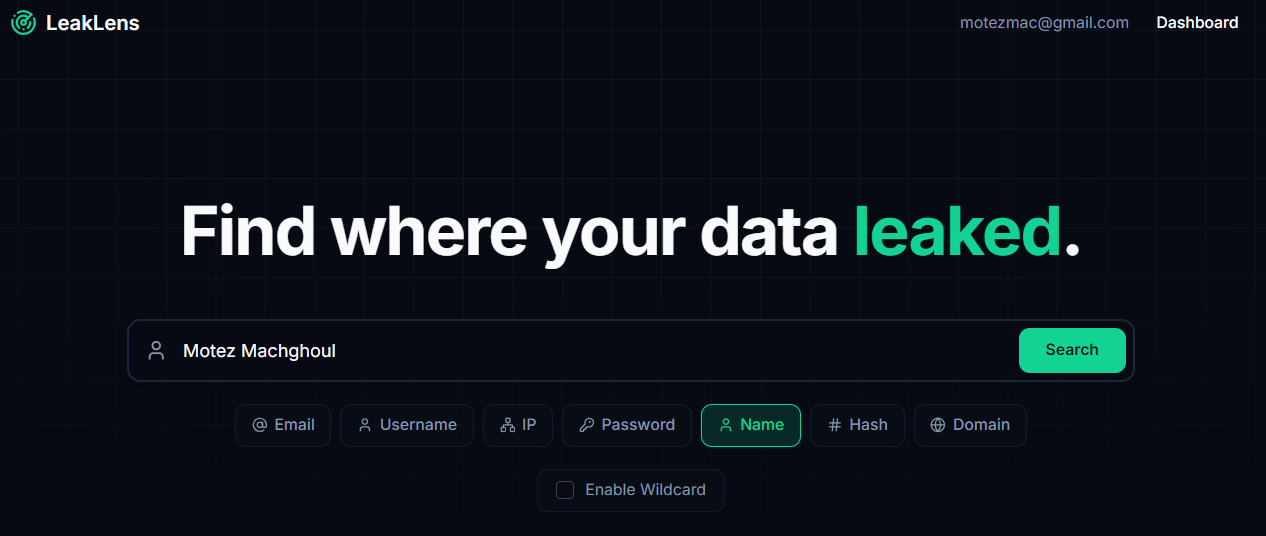
\includegraphics[width=\linewidth,keepaspectratio]{home-auth.png}
\caption{Home page with search interface (authenticated user).}
\label{fig:home}
\end{figure}

\subsection{Search Results}

Search results are displayed as cards grouped by source database. Each card
shows the database name, severity badge (critical/high/medium/low), and
credential fields. Sensitive fields (passwords, hashes) are blurred by
default and can be revealed with a click. A copy button is available for each
field.

\begin{figure}[H]
\centering
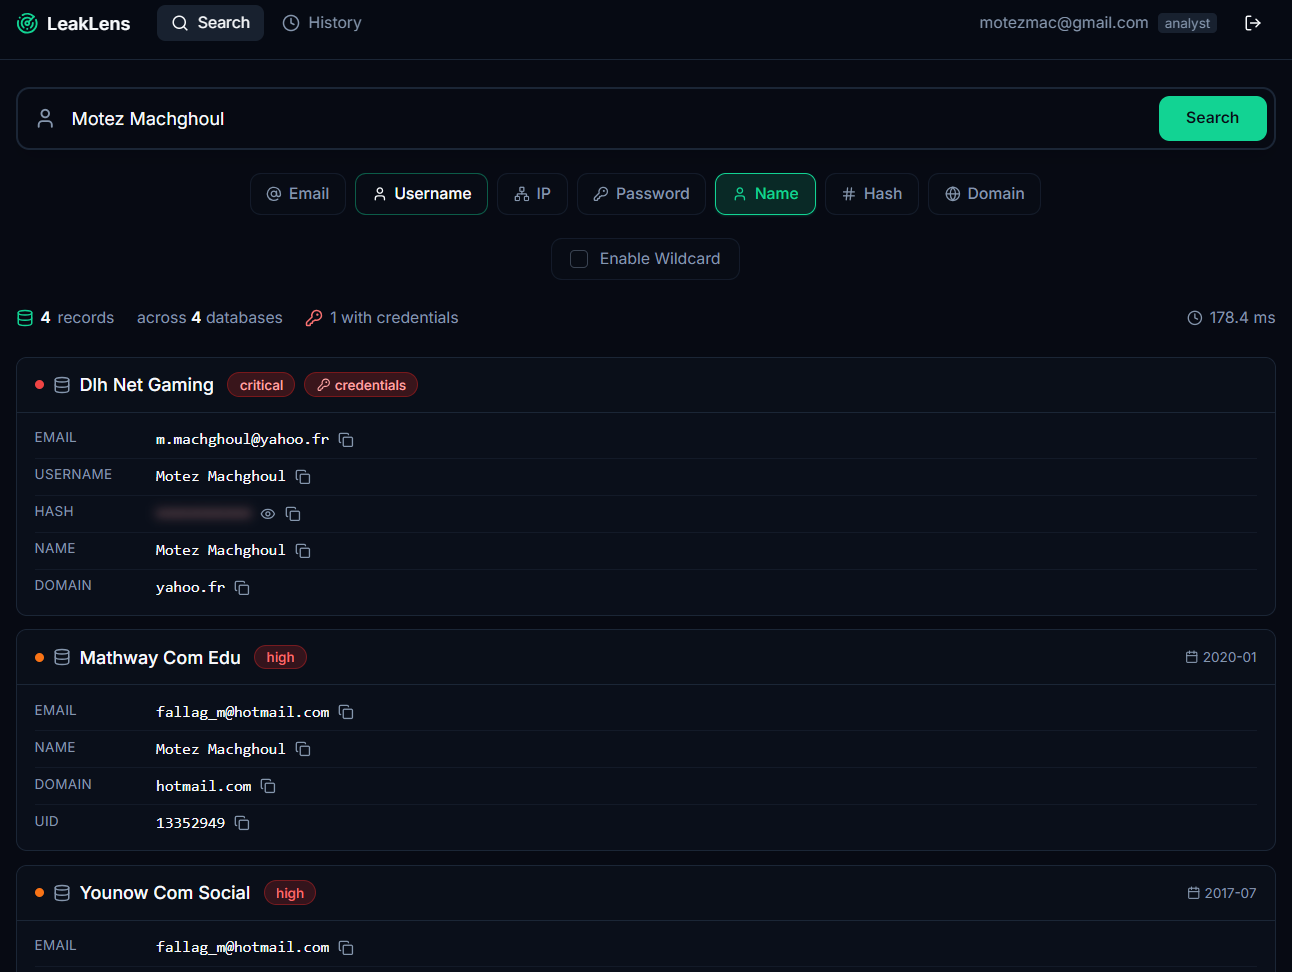
\includegraphics[width=\linewidth,keepaspectratio]{results.png}
\caption{Search results page showing leak records with severity badges.}
\label{fig:results}
\end{figure}

\subsection{Enrichment Panel}

When searching by email or domain, supplementary intelligence is displayed
in a dedicated enrichment panel: subdomain discovery, WHOIS data, and email
reputation scores.

\begin{figure}[H]
\centering
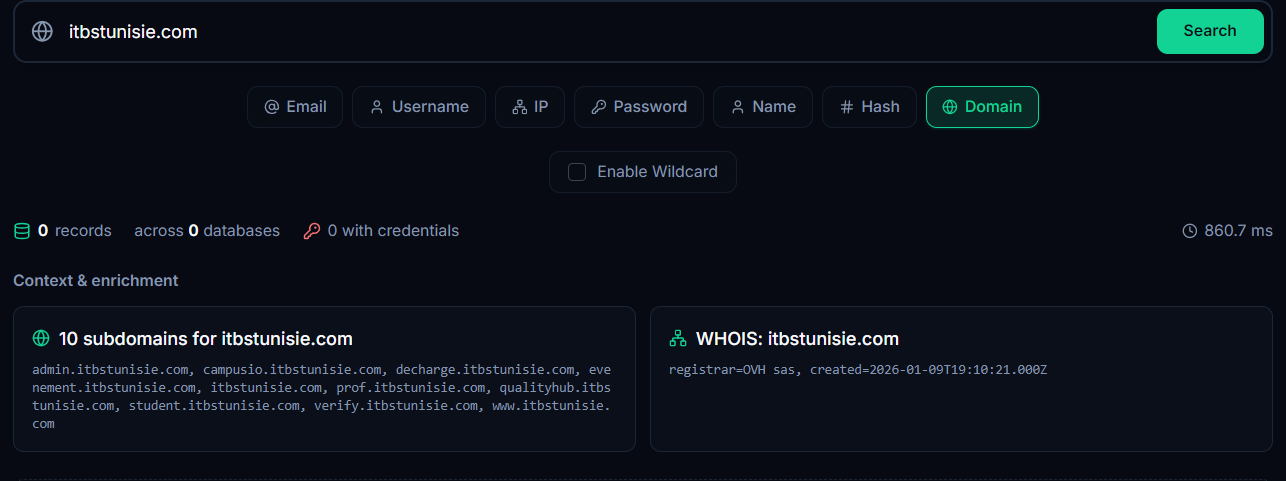
\includegraphics[width=\linewidth,keepaspectratio]{enrichment.png}
\caption{Enrichment panel showing supplementary intelligence.}
\label{fig:enrichment}
\end{figure}

\subsection{Search History}

The history page lists the user's past searches with the query, type,
result count, and timestamp. A ``Search again'' button allows re-running
any past query.

\begin{figure}[H]
\centering
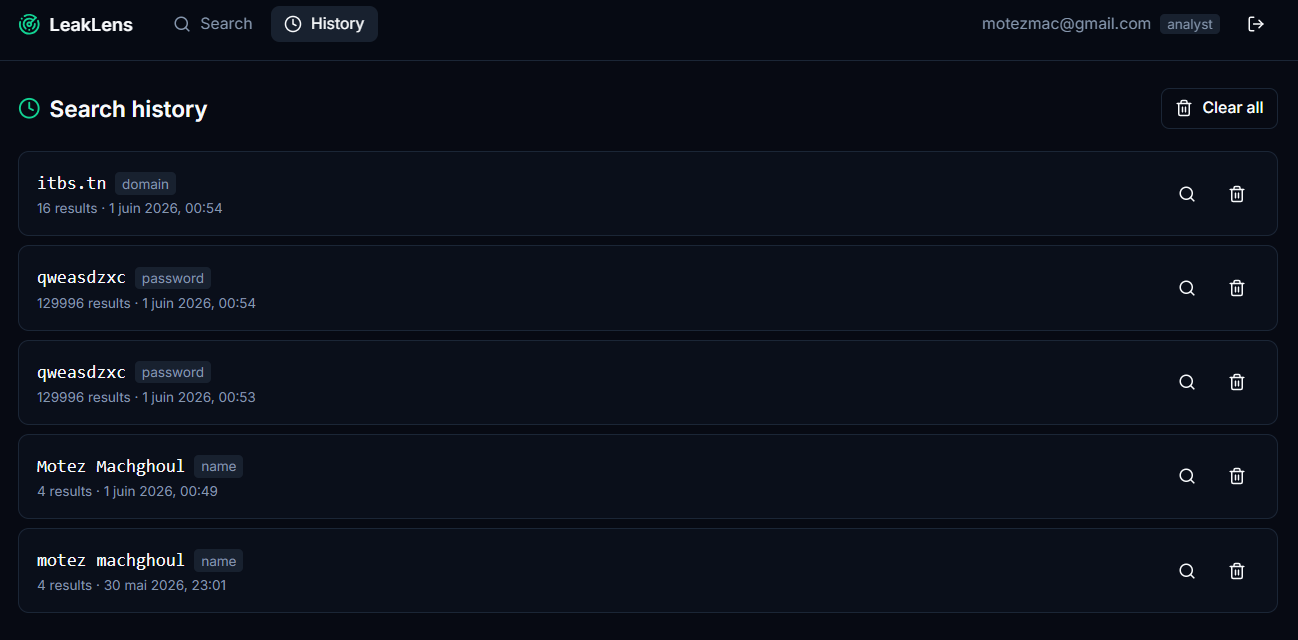
\includegraphics[width=\linewidth,keepaspectratio]{search-history.png}
\caption{Search history page.}
\label{fig:history}
\end{figure}

\FloatBarrier

% ----------------------------------------------------------------------------
\section{Docker Deployment}
\label{sec:docker-deploy}
% ----------------------------------------------------------------------------

The backend is deployed on the VPS using Docker Compose. The following
screenshots document the build process, running containers, and API health
verification.

\subsection{Docker Compose Build}

Production deployment is started with \texttt{docker compose up -d --build}.
The multi-stage Alpine image compiles Python dependencies in a builder stage,
ships a minimal runtime, and starts the FastAPI and PostgreSQL services with
health-check dependencies.

\begin{figure}[H]
\centering
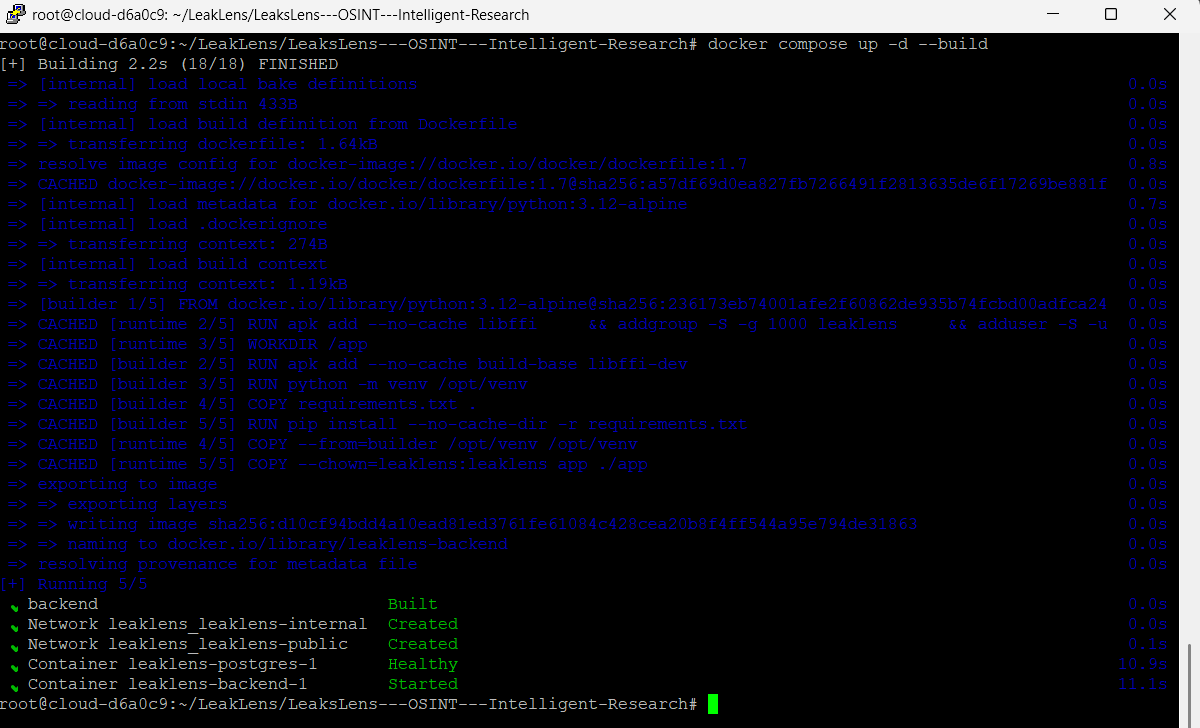
\includegraphics[width=\linewidth,keepaspectratio]{docker-build.png}
\caption{Successful \texttt{docker compose up -d --build} on the VPS.}
\label{fig:docker-build}
\end{figure}

\subsection{Container Status}

Once the stack is running, both containers report a healthy state. PostgreSQL
remains on the internal Docker network; only the FastAPI service is exposed
to the host on port~8500.

\begin{figure}[H]
\centering
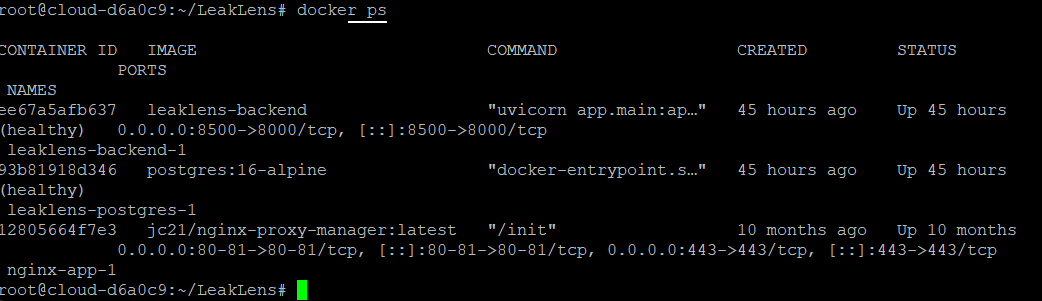
\includegraphics[width=\linewidth,keepaspectratio]{docker-ps.png}
\caption{\texttt{docker ps} output showing \texttt{leaklens-backend-1} and
\texttt{leaklens-postgres-1} in healthy state.}
\label{fig:docker-ps}
\end{figure}

\subsection{Health Check}

The backend exposes a lightweight \texttt{/health} endpoint used by Docker
health checks and for manual verification after deployment.

\begin{figure}[H]
\centering
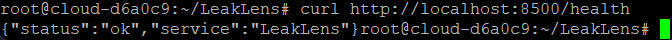
\includegraphics[width=\linewidth,keepaspectratio]{health-check.png}
\caption{Health check response confirming the API is operational.}
\label{fig:health-check}
\end{figure}

\FloatBarrier

% ----------------------------------------------------------------------------
\section{Search Demonstration}
\label{sec:search-demo}
% ----------------------------------------------------------------------------

This section presents two live queries executed against the production
instance. Results illustrate how \leaklens{} surfaces breached credentials and
organizational exposure from Snusbase and enrichment sources.

\subsection{Password Search}

To demonstrate password-type lookup, the query \texttt{'qwerty@'} was submitted. The platform returned
\textbf{748 records} spanning multiple source databases. Each result card
lists the associated email or username, the exposed password field (blurred by
default in the UI), the originating breach compilation, and a severity badge
--- most entries are rated \emph{critical} because plaintext credentials are
present. \figref{fig:password-search} shows a representative subset of these
results; the full result set confirms how widely reused weak passwords such as
\texttt{qwerty} propagate across unrelated services.

\begin{figure}[H]
\centering
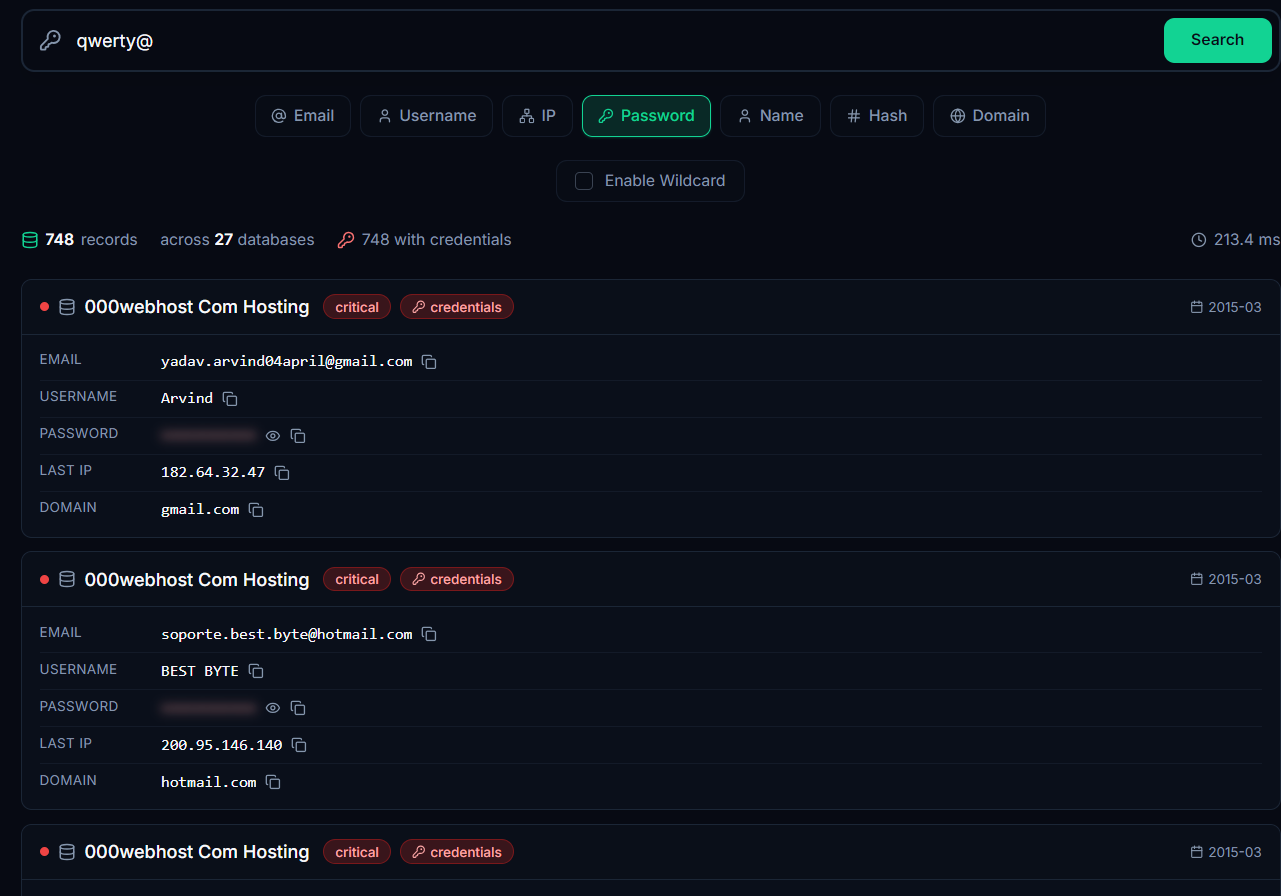
\includegraphics[width=\linewidth,keepaspectratio]{password-search.png}
\caption{Password search for \texttt{qwerty}: 748 leaked credential records
across multiple breach databases.}
\label{fig:password-search}
\end{figure}

\subsection{Domain Search}

A domain search for \texttt{'itbs.tn'} was run to assess exposure tied to an
educational institution. The Search Engine  returned
\textbf{16 breached student records} linked to email addresses under that
domain, together with subdomain and WHOIS context in the enrichment panel.
This type of query helps defenders identify whether institutional accounts
appear in public leak compilations and prioritize password resets or MFA
enforcement for affected users. \figref{fig:search-domain} captures the
domain results and  returned .

\begin{figure}[H]
\centering
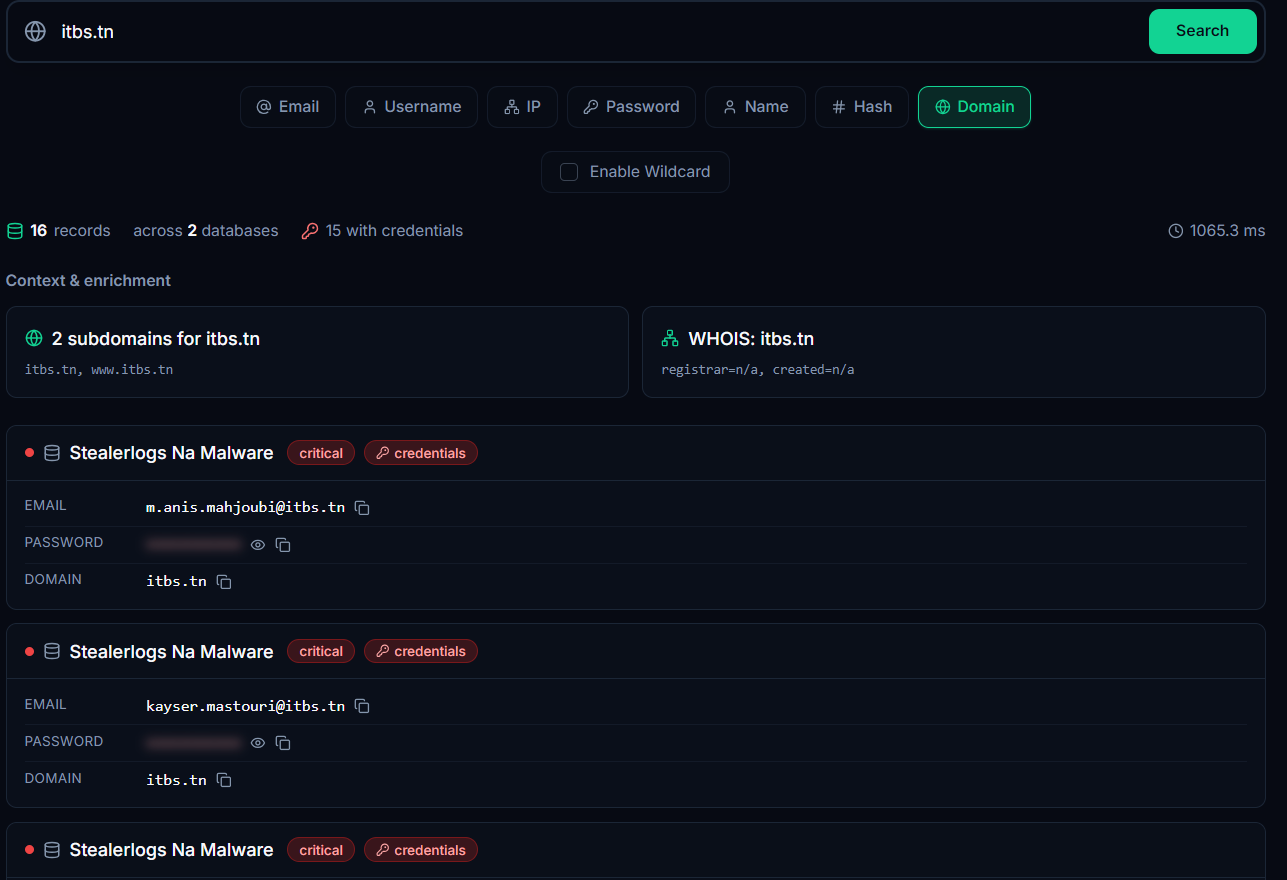
\includegraphics[width=\linewidth,keepaspectratio]{domain-search.png}
\caption{Domain search for \texttt{itbs.tn}: 16 breached student records with
subdomain and WHOIS enrichment.}
\label{fig:search-domain}
\end{figure}

\subsection{Name Search}

An individual or employee can search by full name to discover where their
personal data has appeared in breach compilations. \figref{fig:name-search}
shows a name search performed with the author's own name: the platform returned
matching records exposing an associated email address and password in plaintext,
illustrating how quickly personal exposure can be identified.

\begin{figure}[H]
\centering
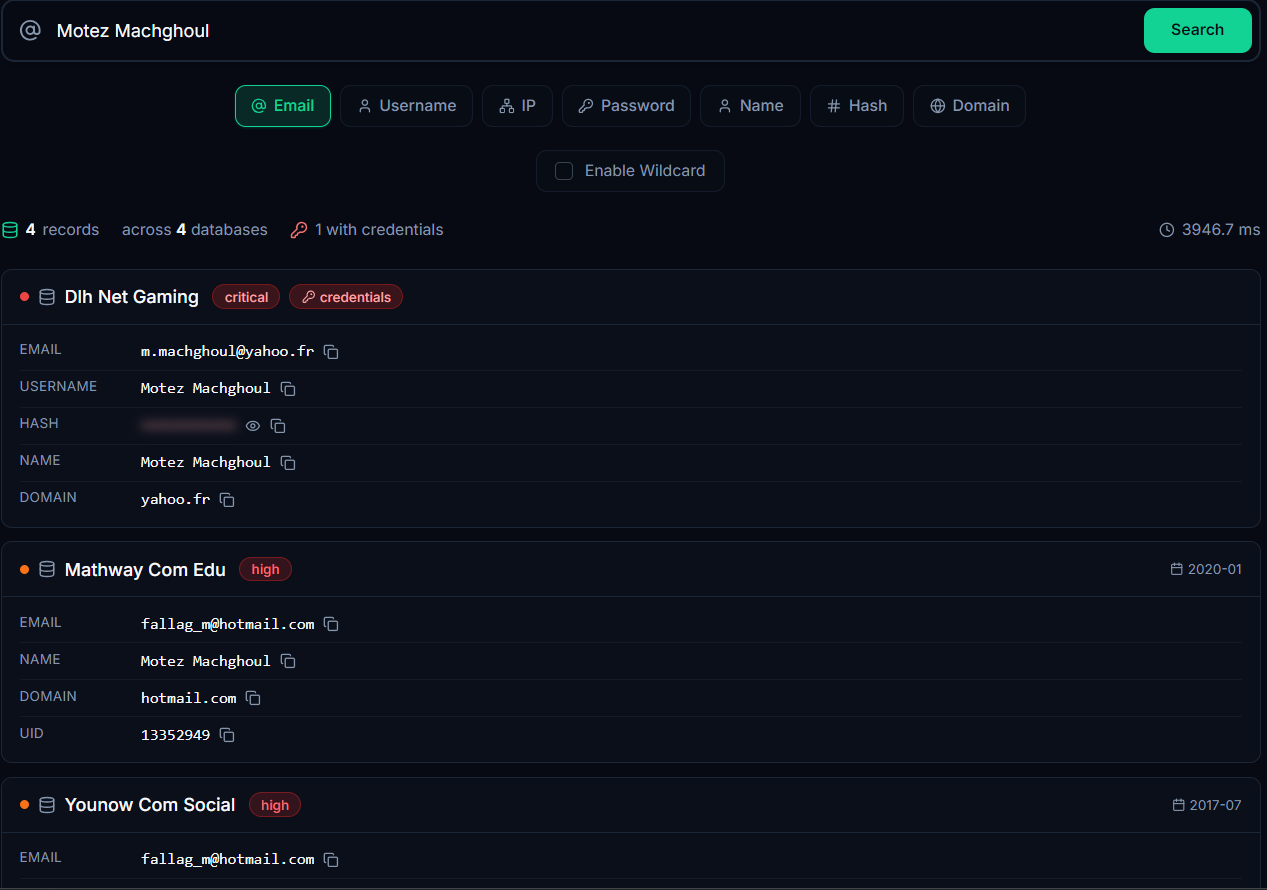
\includegraphics[width=\linewidth,keepaspectratio]{name-search.png}
\caption{Name search revealing leaked email and password associated with the
queried identity.}
\label{fig:name-search}
\end{figure}

\FloatBarrier

% ----------------------------------------------------------------------------
\section*{Conclusion}

This chapter demonstrated the operational \leaklens{} platform through its
user interface, Docker deployment on the VPS, and three live breach searches.
The password query for \texttt{qwerty@} returned 748 credential records across
multiple databases; the domain query for \texttt{itbs.tn} exposed 16 student
accounts; and a name search confirmed personal exposure by surfacing a linked
email and plaintext password. Together, these results confirm that the
end-to-end search pipeline described in earlier chapters works as designed in
production.


% ---- Back matter -----------------------------------------------------------
% ============================================================================
% General Conclusion
% ============================================================================
\chapter*{General Conclusion}
\addcontentsline{toc}{chapter}{General Conclusion}
\markboth{General Conclusion}{}

This end-of-year project resulted in the design, development, and deployment
of \leaklens{}, an OSINT platform for breach-data research. The work covered
requirements analysis, security-oriented architecture, and production
deployment on Vercel and a VPS.

The platform enables analysts to query compromised records across seven search
types, enriched with public intelligence APIs. Its security model combines
JWT authentication, RBAC, invite-only registration, rate limiting, and HTTP
hardening (CSP, HSTS, CORS)---applied as defense-in-depth rather than isolated
controls.

Beyond the technical deliverable, this project consolidated skills directly
relevant to cybersecurity practice:

\begin{itemize}[nosep]
  \item Full-stack development with Next.js and FastAPI;
  \item Application security: JWT, RBAC, anti-enumeration, rate limiting;
  \item Containerization with Alpine Docker builds and Trivy scanning;
  \item External API orchestration (Snusbase, LeakCheck, EmailRep, CertSpotter);
  \item Split deployment across Vercel and a VPS with Nginx Proxy Manager.
\end{itemize}

\section*{Future Improvements}

\begin{enumerate}[nosep]
  \item Custom HTTPS domain with Let's Encrypt via Nginx Proxy Manager;
  \item Local breach-data indexing with Elasticsearch;
  \item Automated CI/CD pipeline (GitHub Actions);
  \item TOTP-based two-factor authentication for analyst accounts;
  \item SIEM integration for search audit logging;
  \item Tor-based monitoring for paste sites and darknet forums.
\end{enumerate}

\vspace{0.8cm}
\begin{center}
\parbox{0.82\textwidth}{\itshape\centering
This project shows that combining OSINT capability with rigorous application
security is achievable at student scale---and that understanding both sides
of the problem is essential for any cybersecurity professional.}
\end{center}

% ============================================================================
% Bibliography
% ============================================================================
\clearpage
\addcontentsline{toc}{chapter}{Bibliography}

\begin{thebibliography}{99}

\bibitem{ibm-breach-report}
IBM Security.
\textit{Cost of a Data Breach Report 2024}.
\url{https://www.ibm.com/reports/data-breach}, 2024.
Accessed May 2026.

\bibitem{moab}
B.~Diachenko.
``Mother of All Breaches: 26 Billion Records Exposed.''
\textit{Security Discovery}, January 2024.
\url{https://www.securitydiscovery.com/}.
Accessed May 2026.

\bibitem{owasp-top10}
OWASP Foundation.
\textit{OWASP Top Ten --- 2021}.
\url{https://owasp.org/www-project-top-ten/}, 2021.
Accessed May 2026.

\bibitem{hibp}
T.~Hunt.
\textit{Have I Been Pwned: Check if your email has been compromised}.
\url{https://haveibeenpwned.com/}, 2013--2026.
Accessed May 2026.

\bibitem{intelx}
IntelligenceX.
\textit{IntelligenceX --- OSINT Search Engine}.
\url{https://intelx.io/}, 2018--2026.
Accessed May 2026.

\bibitem{dehashed}
DeHashed.
\textit{DeHashed --- Breach Search Engine}.
\url{https://www.dehashed.com/}, 2019--2026.
Accessed May 2026.

\bibitem{fastapi-docs}
S.~Ram\'\i rez.
\textit{FastAPI Documentation}.
\url{https://fastapi.tiangolo.com/}, 2019--2026.
Accessed May 2026.

\bibitem{nextjs-docs}
Vercel.
\textit{Next.js Documentation --- The React Framework for the Web}.
\url{https://nextjs.org/docs}, 2016--2026.
Accessed May 2026.

\bibitem{docker-docs}
Docker Inc.
\textit{Docker Documentation --- Build, Ship, Run}.
\url{https://docs.docker.com/}, 2013--2026.
Accessed May 2026.

\bibitem{postgresql-docs}
The PostgreSQL Global Development Group.
\textit{PostgreSQL 16 Documentation}.
\url{https://www.postgresql.org/docs/16/}, 2023.
Accessed May 2026.

\bibitem{sqlalchemy-docs}
M.~Bayer.
\textit{SQLAlchemy Documentation}.
\url{https://docs.sqlalchemy.org/}, 2006--2026.
Accessed May 2026.

\bibitem{jwt-rfc}
M.~Jones, J.~Bradley, N.~Sakimura.
\textit{RFC 7519 --- JSON Web Token (JWT)}.
IETF, May 2015.
\url{https://tools.ietf.org/html/rfc7519}.

\bibitem{bcrypt-paper}
N.~Provos, D.~Mazi\`eres.
``A Future-Adaptable Password Scheme.''
\textit{Proceedings of the USENIX Annual Technical Conference}, 1999.

\bibitem{csp-mdn}
Mozilla Developer Network.
\textit{Content Security Policy (CSP)}.
\url{https://developer.mozilla.org/en-US/docs/Web/HTTP/CSP}, 2024.
Accessed May 2026.

\bibitem{snusbase-docs}
Snusbase.
\textit{Snusbase API Documentation}.
\url{https://docs.snusbase.com/}, 2020--2026.
Accessed May 2026.

\bibitem{osint-framework}
J.~Nordine.
\textit{OSINT Framework}.
\url{https://osintframework.com/}, 2015--2026.
Accessed May 2026.

\bibitem{nist-breach}
National Institute of Standards and Technology.
\textit{NIST SP 800-122: Guide to Protecting the Confidentiality of
Personally Identifiable Information (PII)}.
\url{https://csrc.nist.gov/publications/detail/sp/800-122/final}, 2010.

\end{thebibliography}


\end{document}
